\begin{center}
\indent
\textit{Insiemi, relazioni, funzioni, numeri naturali e principio di induzione, calcolo combinatorio.}
\end{center}

\section{Insiemi}

L'insieme \`e un concetto primitivo senza definizione. Ma definiamo come si fa ad assegnare un insieme. Il modo pi\`u semplice \`e quello di elencarne gli elementi. 
\[
A = \left\{ \text{giallo}, \text{rosso}, \text{blu} \right\}
\]

Un altro modo \`e definendo una propriet\`a.
\[
A = \left\{ x \in X : P(x) \right\}
\]

Un insieme fondamentale \`e quello delle coppie ordinate. $A$, $B$ insiemi. $A \times B =$ insieme delle coppie ordinate.
\[
A \times B = \left\{ (a,b) : a \in A, b \in B \right\}
\]

C'\`e una differenza fondamentale fra insiemi e coppie ordinate.
\begin{gather*}
(a,b) = (c,d) \Leftrightarrow a = c \land b = d \\
\{a,b\} = \{c,d\} \Leftrightarrow (a = c \land b = d) \lor (a = d \land b = c)
\end{gather*}
Il concetto pu\`o essere generalizzato da coppie a terne, quaterne, e in generale $n$-uple.

Una relazione binaria tra due insiemi \`e un sottonisieme di $A \times B$. Il prodotto cartesiano non \`e associativo, ma i due insiemi $A \times B$ e $B \times A$ hanno la stessa cardinalit\`a.

Una funzione da un'insieme $A$ ad un insieme $B$ \`e una terna $(A, B, f)$ o $f : A \to B$, dove $A$ si dice Dominio, $B$ si dice Codominio, ed $f$ \`e una relazione ($f \subseteq A \times B$) t.c. $\forall \ a \in A \ \exists \text{ un solo } b \in B \text{ t.c. } (a,b) \in f$, ossia che $b = f(a)$.

Esiste una funzione da $A = \emptyset$ a $B \neq \emptyset$? S\`i, la funzione $(\emptyset, B, \emptyset)$. Viceversa, una funzione da $A \neq \emptyset$ a $B = \emptyset$ non esiste.

\[
R_1 = \left\{ (m, n) \in \mathbb{N}^2 : m = n^2 \right\}
\]
Non \`e una funzione. Perch\'e? \vspace{3cm}

\[
R_2 = \left\{ (r, s) \in \mathbb{R}^+ \times \mathbb{R} : r = s^2 \right\}
\]
Non \`e una funzione. Perch\'e?
\vspace{3cm}

\[
R_3 = \left\{ (r, s) \in \mathbb{R}^+ \times \mathbb{R}^+ : r = s^2 \right\}
\]
\`E una funzione. Perch\'e?
\vspace{3cm}

\begin{defn}
Due funzioni sono uguali solo se coincidono come terne.
\end{defn}

Per definire una funzione bisogna definire l'insieme del Dominio, definire l'insieme del Codominio, e una relazione che gode della propriet\`a che ogni elemento del dominio ha una sola immagine.

Sia $f : A \to B$ una funzione, $Im_f =$ immagine di $f$.
\[
Im_f = \left\{ b \in B : \exists \ a \in A \text{ t.c. } f(a) = b \right\}
\]

\[
f : \mathbb{N} \to \mathbb{N} \text{ t.c. } \forall \ n \in \mathbb{N} \ f(n) = 
\begin{cases} 
n - 1 & \text{se $n$ \`e pari} \\
n + 1 & \text{se $n$ \`e dispari}
\end{cases}
\]
Non \`e una funzione perch\'e lo zero non ha immagine.

\[
f : \mathbb{R} \to \mathbb{R} \text{ t.c. } \forall \ r \in \mathbb{R} \ f(r) = 
\begin{cases}
r^2 + 1 & \text{ se r $\leq$ 0 } \\
r & \text{ se r $\geq$ 0} 
\end{cases}
\]
Non \`e una funzione perch\'e lo zero ha due immagini.

\subsection{Propriet\`a delle funzioni}

\begin{description}
\item[Suriettiva\label{itm:suriettiva}] Ogni elemento di $B$ \`e immagine di un elemento di $A$, ossia $Im_f = B$.
\item[Iniettiva\label{itm:inettiva}] Due elementi diversi di $A$ non hanno la stessa immagine.
\end{description}

\`E pi\`u facile dimostrare l'iniettivit\`a di una funzione in un altro modo.

$f$ \`e iniettiva $\Leftrightarrow a, a' \in A $, se $ f(a) = f(a')$ allora $a = a'$.

Una funzione iniettiva e suriettiva \`e detta ``biunivoca''.

\[
f: \mathbb{R} \times \mathbb{R} \to \mathbb{R} \text{ t.c. } f(x,y) = \sqrt{2}x + y
\] 
Non \`e iniettiva, perch\'e $(1,0)$ e $(0,\sqrt{2})$ hanno la stessa immagine. \`E suriettiva.

\[
\forall \ r \in \mathbb{R} \ \exists \ (x,y) \in \mathbb{R} \times \mathbb{R} \text{ t.c. } f(x,y) = \sqrt{2} x + y = r
\]
Basta scegliere $(0,r)$ e $f(0,r) = r$.

Determiniamo le immagini della funzione per i Domini dati.

\begin{gather*}
A = \left\{ \left( a, - \sqrt{2}a\right) : a \in \mathbb{R}  \right\} \\
f(A) = \left\{ r \in \mathbb{R} : \exists \ (a, - \sqrt{2}a) \text{ t.c. } f(a, - \sqrt{2} a) = r \right\} = \left\{ 0 \right\}
\end{gather*}
\begin{gather*}
C = \left\{ (a, \sqrt{2} b) : a, b \in \mathbb{Z} \right\} \\
f(C) = \left\{ r \in \mathbb{R} : \exists \ (a, \sqrt{2} b) \text{ t.c. } f(a, \sqrt{2}b) = r \right\} \\
r = f(a, \sqrt{2} b) = \sqrt{2} a + \sqrt{2} b = \sqrt{2} (a + b) \\
(a+b) \in \mathbb{Z} \\
r \in \sqrt{2} \mathbb{Z} = \left\{z : z = \sqrt{2} t \text{ con } t \in \mathbb{Z} \right\}
\end{gather*}

L'insieme delle funzioni da $A$ in $B$ si indica con $B^A$. Questo insieme verifica tutte le propriet\`a delle potenze. Alla somma corrisponde l'unione, al prodotto corrisponde il prodotto cartesiano. Inoltre $|B| = m$, $|A| = n$, $|B^A| = m^n$.

\subsubsection{Composizione}

Date le funzioni $f : A \to B$ e $g : B \to C$, la composizione $g \circ f : A \to C$ \`e definita come:
\[
\forall \ a \in A , \ {g \circ f}(a) = g(f(a))
\]
L'operazione di composizione \`e una funzione $f : B^A \times C^B \to C^A$.

\begin{description}
  \item[Inversa destra] Data $f : X \to Y$, $g : Y \to X$ \`e un'inversa destra se $f \circ g = id_Y$ (funzione identit\`a)
  \item[Inversa sinistra] Data $f : X \to Y$, $g : Y \to X$ \`e un'inversa destra se $g \circ f = id_X$
\end{description}

\section{Relazioni su un insieme}

Una relazione su un insieme $A$ \`e un sottoinsieme $R \subseteq A \times A$. I tipi di relazioni su un insieme sono due:

\begin{description}
    \item[Relazioni d'ordine] Si indica con $\le$, $a \leq b$ indica che $a$ \`e in relazione con $b$. Propriet\`a:
    \begin{description}
        \item [Riflessiva] $\forall \ x \in A : x \leq x$
        \item [Antisimmetrica] $\forall \ x, y \in A \text{ se } x \leq y \text{ e }  y \leq x \Rightarrow x = y$
        \item [Transitiva] $\forall \ x, y, z \in A \text{ se } x \leq y \text{ e } y \leq z \Rightarrow x \leq z$
    \end{description}
    \item[Relazioni di equivalenza] Si indica con $\varepsilon$, $a \varepsilon b$ indica che $a$ \`e in relazione con $b$. Propriet\`a:
    \begin{description}
      \item [Riflessiva] (vedi sopra), posso scriverla anche come $\forall \ a \in A \ \exists \ x \in A : a \varepsilon x$
      \item [Simmetrica] $x \varepsilon y \Rightarrow y \varepsilon x$.
      \item [Transitiva] (vedi sopra)
    \end{description}
\end{description}

Le tre propriet\`a di una relazione d'ordine (riflessiva, antisimmetrica e transitiva) sono \textit{indipendenti}, ossia nessuna propriet\`a deriva dalle altre. Per dimostrarlo, forniamo degli esempi.
\begin{itemize}
  \item Antisimmetrica e transitiva, ma non riflessiva: $x \le y \Leftrightarrow x \neq y$. \textit{A me sembra sia invece simmetrica e transitiva. $x \le y \Leftrightarrow x < y$ \`e antisimmetrica e transitiva, essendo una relazione di ordine stretto.}
  \item Riflessiva e transitiva, ma non antisimmetrica: definita su $A = $ \{insieme di persone\}, $ \ a R b \Leftrightarrow a$ ha la stessa et\`a di $b$.
  \item Riflessiva e antisimmetrica, ma non transitiva: definita su $\mathbb{N}, x R y \Leftrightarrow x - y \le 2$.
\end{itemize}

\textbf{Esercizio:} trovare altri esempi.

\vspace{5cm}

Anche le propriet\`a delle relazioni d'equivalenza sono indipendenti. Potrebbe sembrare che la propriet\`a riflessiva sia conseguenza della propriet\`a simmetrica e della propriet\`a transitiva.
\begin{gather*}
x \varepsilon y \Rightarrow y \varepsilon x \text{ per la propriet\`a simmetrica} \\
x \varepsilon y , y \varepsilon x \Rightarrow x \varepsilon x \text{ per la propriet\`a transitiva}
\end{gather*}
L'errore \`e che $x \varepsilon y$ non \`e dato \textit{per ogni $x$}: la relazione \`e riflessiva se $\forall \ x \in A \ \exists \ y : x \varepsilon y \Leftrightarrow $ la relazione \`e riflessiva.

Altri esempi di relazioni con solo alcune delle propriet\`a delle relazioni d'ordine:
\begin{itemize}
  \item Relazione transitiva e simmetrica, ma non riflessiva:
  \[
  (m, n) \in \mathbb{N} \times \mathbb{N}, \ (m,n) R (p, q) \Leftrightarrow \frac{m}{p} = \frac{n}{q}
  \]
  La coppia $(m,0)$ non \`e in relazione con nessuno se $m \neq 0$.
  \item Relazione riflessiva e transitiva, ma non simmetrica: una qualsiasi relazione d'ordine (essendo tutte antisimmetriche).
  \item Relazione riflessiva, simmetrica ma non transitiva: dato l'insieme delle rette nello spazio euclideo, $r R s \Leftrightarrow r $ \`e complanare a $s$ ($r // s$ - $r$ parallela ad $s$ - oppure $r \cap s = \{ P \}$ - si incontrano in un punto).
\end{itemize}

\textbf{Esercizio}: verificare le propriet\`a delle seguenti relazioni.
\begin{itemize}
  \item Parallelismo tra rette dello spazio \vspace{3cm}
  \item $\mathbb{N} \times \mathbb{N}, (m, n) \rho (p, q) \Leftrightarrow (m + q) = (p + n)$, ossia $m - n = p - q$. \vspace{3cm}
  \item $a, b \in \mathbb{Z}, a \equiv_n b \Leftrightarrow n | (a - b) \Leftrightarrow (a-b) = k n$ (congruenza modulo $n \in \mathbb{N}, n \ge 2$) \vspace{3cm}
  \item Data una funzione $f: A \to B $, $ \varepsilon_f = $ \`e relazione di equivalenza individuata da $f$, detta ``nucleo di $f$''. \`E una relazione su $A$ t.c. $a, a' \in A, a \varepsilon_f a' \Leftrightarrow f(a) = f(a')$. \vspace{3cm}
\end{itemize}

Data una relazione $R \subseteq A \times B$, possiamo definire $R^{\ast} = $ relazione duale di $R$. Due elementi $(a,b) \in A \times B$ sono $a \ R^{\ast} \ b \Leftrightarrow b \ R \ a$. Ad esempio, se $A = $ insieme di persone e $R = a $ figlio di $b$, la relazione duale \`e $R^{\ast} = b $ \`e genitore di $a$.

La duale di una relazione d'ordine \`e ancora una relazione d'ordine, e viene tipicamente indicata con $\geq$.

La coppia $(P, \leq)$ data dall'insieme $P \neq \emptyset$ con una relazione d'ordine $\le$ si dice insieme parzialmente ordinato.

Se $\forall \ x, y \in P$ e si ha che $x \leq y \lor y \leq x$, $(P, \leq)$ si dice linearmente ordinato (o totalmente ordinato).

L'insieme dei numeri naturali $\mathbb{N}$ con la relazione d'ordine naturale $(\mathbb{N}, \leq)$ \`e totalmente ordinato. Ma possiamo prendere anche l'insieme dei numeri naturali con la relazione di divisibilit\`a $(\mathbb{N}, |)$, ossia $m | n \Leftrightarrow m \text{ divide } n \Leftrightarrow \exists \ k \in \mathbb{N}$ t.c. $n = k \ m$. Rispetto a questa relazione d'ordine, $\mathbb{N}$ non \`e totalmente ordinato.

L'insieme delle parti di un insieme $\Gamma$ qualunque con la relazione ``\`e sottoinsieme di'' $\left(\mathbb{P}(\Gamma), \subseteq \right)$ \`e un insieme parzialmente ordinato. 

Come si costruisce in modo naturale una relazione su un prodotto cartesiano? Ad esempio, prendo la relazione d'ordine naturale sui reali $(\mathbb{R}, \leq)$ e $(\mathbb{R}^2, \leq)$, ho $(a,b) \leq (c,d) \Leftrightarrow a \leq c \land b \leq d$.

\[
B = \{ n \in \mathbb{N} : n = 2^r 3^s, r, s \in \mathbb{N}\}
\]
Definisco $\rho$ su $B$ come $2^r 3^s \leq 2^t 3^u \Leftrightarrow r \leq t \land s \leq u$. \`E una relazione d'ordine parziale. Perch\'e?
\vspace{3cm}

\begin{defn}[Ordine naturale sul prodotto cartesiano]
Dati due insiemi parzialmente ordinati $(P_1, \le_1)$ e $(P_2, \le_2)$, posso definire naturalmente una relazione d'ordine sul prodotto dei due insiemi $(P_1 \times P_2, \le)$ come:
\[
(x_1, x_2) \le (y_1, y_2) \Leftrightarrow x_1 \le_1 y_1 \land x_2 \le_2 y_2
\]
Si pu\`o generalizzare anche a $(P^n, \le)$, prendendo le $n$-uple al posto delle coppie.
\end{defn}

\begin{defn}[Ordine fra funzioni]\label{ordine_funzioni}
Se prendo un insieme parzialmente ordinato $(P, \le)$ e un insieme qualsiasi $A$, posso definire una relazione su $(P^A, \le)$ (ricordando che $P^A$ \`e l'insieme di tutte le funzioni da $A$ a $P$). Come faccio a dire che date $f, g \in P^A \ f \le g$? Se $\forall \ a \in A \ f(a) \le g(a)$.
\end{defn}

\subsection{Diagramma di Hasse}

Dato un insieme e una relazione di ordine parziale su di esso $(A, \leq)$, rappresento gli elementi di $A$ con dei punti sul piano. Posiziono il punto $x \in A$ pi\`u in basso di $y \in A$ se $x \leq y$. Congiungo con un segmento gli elementi $x, y$ se $y$ ``copre'' $x$, ossia se l'intervallo individuato dagli estremi $x, y = [x, y] = \left \{ z \in A : x \leq z \leq y \right \}$ contiene solo $x$ ed $y$. Si dice $y$ ``copre'' $x$ o $x$ ``\`e coperto'' da $y$ e si indica con $x \covers \ y$.

\begin{figure}[ht]
\centering
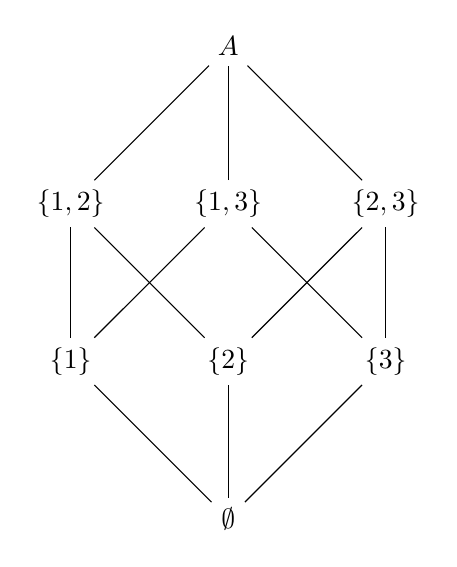
\begin{tikzpicture}
  \node (A) {$A$};
  \node (13) [below of=A, node distance=2cm] {$\{1,3\}$};
  \node (12) [left of=13, node distance=2cm] {$\{1,2\}$};
  \node (23) [right of=13, node distance=2cm] {$\{2,3\}$};
  \node (1) [below of=12, node distance=2cm] {$\{1\}$};
  \node (2) [below of=13, node distance=2cm] {$\{2\}$};
  \node (3) [below of=23, node distance=2cm] {$\{3\}$};
  \node (O) [below of=2, node distance=2cm] {$\emptyset$};
  \path[-]  (O) edge node {} (1)
            (O) edge node {} (2)
            (O) edge node {} (3)
            (1) edge node {} (12)
            (1) edge node {} (13)
            (2) edge node {} (12)
            (2) edge node {} (23)
            (3) edge node {} (13)
            (3) edge node {} (23)
            (12) edge node {} (A)
            (13) edge node {} (A)
            (23) edge node {} (A)
            ;
\end{tikzpicture}
\caption{Diagramma di Hasse della relazione $(\mathbb{P}(A), \subseteq)$ sull'insieme $A = \{1, 2, 3\}$}
\end{figure}

\begin{figure}[ht]
\centering
\begin{tikzpicture}
  \node (24) {24};
  \node (8) [below left of=24, node distance=2cm] {8};
  \node (12) [below right of=24, node distance=2cm] {12};
  \node (4) [below left of=12, node distance=2cm] {4};
  \node (6) [below right of=12, node distance=2cm] {6};
  \node (2) [below left of=6, node distance=2cm] {2};
  \node (3) [below right of=6, node distance=2cm] {3};
  \node (1) [below left of=3, node distance=2cm] {1};
  \path[-]  (24) edge node {} (8)
            (24) edge node {} (12)
            (8) edge node {} (4)
            (12) edge node {} (4)
            (12) edge node {} (6)
            (4) edge node {} (2)
            (6) edge node {} (2)
            (6) edge node {} (3)
            (2) edge node {} (1)
            (3) edge node {} (1)
            ;
\end{tikzpicture}
\caption{Diagramma di Hasse della relazione $(A,|)$ sull'insieme $A = \{n \in \mathbb{N} : n | 24\} = \{ 1, 2, 3, 4, 6, 8, 12, 24 \} $}
\end{figure}

\begin{theorem}
Ogni insieme \`e suscettibile di un ordine totale, ossia si pu\`o totalmente ordinare.
\end{theorem}

\textbf{Esercizio:} determinare due ordini diversi su $\mathbb{Q}$.

\vspace{5cm}

\subsection{INF e SUP}

\begin{defn}[INF]
Dato un insieme $(P, \leq)$ parzialmente ordinato, e due elementi $x,y \in P$, si dice INF di $x$ e $y$ l'elemento $\inf(x,y)$ tale che:
\begin{description}
    \item[INF1\label{itm:inf1}] $\inf(x,y) \leq x $ e $ \inf(x,y) \leq y$
    \item[INF2\label{itm:inf2}] $z \in P$, se $ z \leq x, y \Rightarrow z \leq \inf(x,y)$
\end{description}
\end{defn}
\begin{defn}[SUP]
Analogamente possiamo definire il SUP di $x,y$, un elemento di P che si indica con $\sup(x,y)$ tale che:
\begin{description}
    \item[SUP1\label{itm:sup1}] $\sup(x,y) \geq x $ e $ \sup(x,y) \geq y$
    \item[SUP2\label{itm:sup2}] $z \in P$, se $ z \geq x, y \Rightarrow z \geq \sup(x,y)$
\end{description}
\end{defn}

Ossia, $\inf(x,y)$ \`e il pi\`u grande dei minoranti di $x,y$ e $\sup(x,y)$ \`e il pi\`u piccolo di tutti i maggioranti di $x, y$.

Prendiamo l'insieme $\Gamma$, il suo insieme delle parti e la relazione ``\`e sottoinsieme di'' $(P(\Gamma),\subseteq)$, e due sottoinsiemi $A, B \subseteq \Gamma$, l'$\inf(A,B) = A \cap B$. Il $\sup(A,B) = A \cup B$.

Prendiamo $(\mathbb{N},|)$ e due elementi $m, n$. L'$\inf(m,n) = \operatorname{MCD}(m,n)$, mentre il $\sup(m,n) = \operatorname{mcm}(m,n)$.

\section{Reticoli}
\begin{defn}
L'insieme parzialmente ordinato $(L, \leq)$ \`e un reticolo se $\forall \ x, y \in L $ esiste $\inf(x,y)$ ed esiste $\sup(x,y)$.
\end{defn}

Posso interpretare i reticoli anche come strutture algebriche. Si possono definire due operazioni su $L$. 

\begin{defn}[Operazione di $\inf$]
Indicata con $\wedge: L \times L \to L$, definita come $ \forall \ (x,y) \in L \times L , \ x \wedge y = \inf(x,y) $.
\end{defn}
\begin{defn}[Operazione di $\sup$]
L'operazione di $\sup $, indicata con $ \vee: L \times L \to L$, definita come $\forall \ (x,y) \in L \times L , \ x \vee y = \sup(x,y)$.
\end{defn}

Ho definito quindi la struttura algebrica $(L, \wedge, \vee)$. Le due operazioni hanno le seguenti propriet\`a, dette \label{proprieta_dei_reticoli} \textbf{propriet\`a dei reticoli}:
\begin{description}
    \item[R1\label{itm:r1}] Idempotenza: $x \wedge x = x ; \ x \vee x = x$.
    \item [R2\label{itm:r2}] Commutativa: $x \wedge y = y \wedge x ; \ x \vee y = y \vee x$.
    \item [R3\label{itm:r3}] Associativa: $x \wedge ( y \wedge z) = (x \wedge y) \wedge z; \ x \vee ( y \vee z) = (x \vee y) \vee z$.
    \item [R4\label{itm:r4}] Assorbimento: $x \wedge (x \vee y) = x ; \ x \vee ( x \wedge y) = x$.
\end{description}
Sono le propriet\`a classiche dell'unione e dell'intersezione.

\begin{proof}[Dimostrazione della propriet\`a \ref{itm:r3}]
Equivale a dimostrare, per doppia inclusione, che $x \wedge ( y \wedge z) \leq (x \wedge y) \wedge z$ e che $(x \wedge y) \wedge z \leq x \wedge ( y \wedge z)$. La prima parte equivale a dire che
\[
x \wedge (y \wedge z) \leq 
\begin{cases}
(x \wedge y) \\
 z
 \end{cases}
\]
Il primo caso equivale a dimostrare che
\[
x \wedge (y \wedge z) \leq x, y \Rightarrow x \wedge (y \wedge z) \leq x \wedge y
\]
Il secondo caso si dimostra subito perch\'e $y \wedge z \leq z, y \Rightarrow y \wedge z \leq z$ \`e vero per definizione di $\inf$. 
\end{proof}

\begin{theorem}
Data una struttura algebrica $(L, \wedge, \vee)$ verificante le quattro propriet\`a dei reticoli, \`e possibile definire su $L$ una relazione d'ordine $\le$ t.c. $ x \wedge y = \inf(x,y) $ e $ x \vee y = \sup(x,y) $ in $ (L, \le)$, ossia $x \le y \Leftrightarrow x \wedge y = x $ (o anche $ x \vee y = y$).
\end{theorem}
\begin{proof}
Dimostriamo che \`e una relazione d'ordine.
\begin{itemize}
    \item Propriet\`a riflessiva: $x \le x$ per \ref{itm:r1}.
    \item Antisimmetrica: $\forall \ x, y \in A \text{ se } x \leq y \text{ e }  y \leq x \Rightarrow x = y$. Dimostrazione: $x \le y \Rightarrow x \wedge y = x$, e $y \le x \Rightarrow y \wedge x = y$. Per \ref{itm:r2} $x = x \wedge y = y \wedge x = y$, per cui $x = y$.
    \item Transitiva: $\forall \ x, y, z \in A \text{ se } x \leq y \land y \leq z \Rightarrow x \leq y$. Dimostrazione: $x \le y \Rightarrow x \wedge y = x$, $y \le z \Rightarrow y \wedge z = y$, da cui $x \le z$. Devo quindi dimostrare che $x \wedge z = x$, quindi che $(x \wedge y) \wedge z = x$. Per \ref{itm:r3} $(x \wedge y) \wedge z = x \wedge (y \wedge z) = x \wedge y = x$. 
\end{itemize}
Rimane da dimostrare che $x \wedge y = \inf(x,y)$. Devo dimostrare due cose:
\begin{enumerate}
    \item $x \wedge y \le x, y$. Infatti $(x \wedge y) \wedge x = (x \wedge y) \Rightarrow (x \wedge y) \le x$, e analogamente $x \wedge y \le y$.
    \item $z \le x, y \Rightarrow z \le (x \wedge y)$. La tesi mi dice che $z \wedge x = z$ e che $z \wedge y = z$. Devo dimostrare quindi $z \wedge (x \wedge z) = z \wedge z = z$.
\end{enumerate}
\end{proof}

\begin{lem}\label{dual}
$ x \le y \Leftrightarrow x \vee y = y $
\end{lem}
\begin{proof}[Dimostrazione del lemma \ref{dual}]
Sostituendo in $x \wedge y = x$ in $ x \vee y $ otteniamo $ (x \wedge y) \vee y = y $, per la propriet\`a \ref{itm:r4}.
\end{proof}
Per dimostrare $x \vee y = \sup(x,y)$ basta sfruttare il lemma \ref{dual}, ripercorrendo le stesse tappe e sostituendo $\sup$ al posto di $\inf$.

I reticoli possono quindi essere visti come strutture algebriche in cui le operazioni sono l'$\inf$ e il $\sup$, o come insiemi parzialmente ordinati.

Ci sono altre due propriet\`a dei reticoli:
\begin{description}
  \item [R5\label{itm:isotoniche}] Le relazioni sono \textit{isotoniche}.
  \[
  x \le y, z \in L \Rightarrow 
  \begin{cases}
  x \wedge z \le y \wedge z \\ 
  x \vee z \le y \vee z
  \end{cases}
  \]
  \item [R6\label{itm:disuguaglianza_distributiva}] Disuguaglianza distributiva. In ogni reticolo $(L, \le) \ \forall \ x, y, z \in L $ si ha:
  \[
  x \vee (y \wedge z) \le (x \vee y) \wedge (x \vee z)
  \]
\end{description}

\begin{proof}[Dimostrazione di \ref{itm:isotoniche}]
Devo dimostrare che $ (x \wedge z) \wedge (y \wedge z) = x \wedge z $.
Per ipotesi $x \le y \Rightarrow x \wedge y = x$.
\begin{multline*}
(x \wedge z) \wedge (y \wedge z) = \\
(x \wedge z) \wedge (z \wedge y) = \\
x \wedge (z \wedge z) \wedge y = \\
(x \wedge z) \wedge y = \\
(x \wedge y) \wedge z = \\
 x \wedge z
\end{multline*}
\end{proof}
\begin{proof}[Dimostrazione di \ref{itm:disuguaglianza_distributiva}]
Per definizione di $\inf$ bisogna dimostrare:
\[
x \vee (y \wedge z) \le 
\begin{cases}
(x \vee y) \\
(x \vee z)
\end{cases}
\]
Poich\`e $\vee$ \`e un'operazione isotonica:
\[
(y \wedge z) \le y \Rightarrow x \vee (y \wedge z) \le x \vee y
\]
\end{proof}

\subsection{Teorema di dualit\`a}
Data una stringa $E(\wedge, \vee)$ contenente gli elementi del reticolo, $\wedge, \vee, (, )$, posso creare la sua stringa duale $E^{\ast} (\vee, \wedge)$ in cui ogni $\wedge$ \`e sostituita da $\vee$, e le relazioni d'ordine sono scambiate.
\begin{gather*}
(x \wedge y) \vee y = E(\wedge, \vee) \\
(x \vee y) \wedge y = E^{\ast} (\vee, \wedge)
\end{gather*}
Vediamo che le propriet\`a dei reticoli sono formule duali.

Perch\`e bisogna scambiare le relazioni d'ordine? Dato un reticolo $(L, \le)$ e il suo duale $(L, \ge)$, il $\sup^{\ast} (x,y) = \inf(x,y)$, e l'$\inf^{\ast}(x,y) = \sup(x,y)$.

\begin{theorem}
Se in un reticolo $(L, \le)$ \`e vero un enunciato $\xi$ relativo a stringhe del tipo $E(\wedge, \vee) \Rightarrow $ \`e vero l'enunciato duale $\xi^{\ast}$ di $\xi$ che si ottiene da $\xi$ sostituendo ad ogni stringa $E(\wedge, \vee)$ la stringa $E^{\ast}(\vee, \wedge)$, e se $E_i (\wedge, \vee) \le E_2 (\wedge, \vee)$, allora $E_i^{\ast} (\vee, \wedge) \ge E_2^{\ast} (\vee, \wedge)$.
\end{theorem}
Ogni volta che dimostro un teorema sui reticoli, \`e vero anche il teorema duale. 

La duale della disuguaglianza distributiva \`e:
\[
x \wedge (y \vee z) \ge (x \wedge y) \vee (x \wedge z)
\]
Che \`e anche la propriet\`a di disuguaglianza distributiva in $(L^{\ast}, \ge)$.

\textbf{Esercizio:} $\xi$: in un reticolo $(L, \le)$ si ha che $x \le z, y \in L \Rightarrow x \vee (y \wedge z) \le (x \vee y) \wedge z$ (disuguaglianza modulare). Dimostrarlo.

\vspace{5cm}

\begin{defn}[Reticolo distributivo]
Se in $(L, \le)$ vale l'identit\`a $x \wedge (y \vee z) = (x \wedge y) \vee (x \wedge z)$, il reticolo si dice distributivo. Vale anche la duale.
\end{defn}

Ogni reticolo distributivo \`e modulare. Esistono reticoli modulari ma non distributivi.

\begin{figure}[ht]
\centering
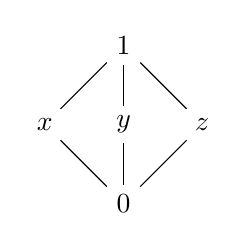
\begin{tikzpicture}
  \node (1) {1};
  \node (y) [below of=1] {$y$};
  \node (x) [left of=y] {$x$};
  \node (z) [right of=y] {$z$};
  \node (0) [below of=y] {0};
  \path[-]  (1) edge node {} (x)
            (1) edge node {} (y)
            (1) edge node {} (z)
            (x) edge node {} (0)
            (y) edge node {} (0)
            (z) edge node {} (0)
            ;
\end{tikzpicture}
\caption{\label{fig:mod_not_distr}Reticolo modulare ma non distributivo}
\end{figure}
Prendiamo ad esempio il reticolo in figura \ref{fig:mod_not_distr}: $(x \wedge y) \vee z = 0 \vee z = z$, $(x \vee z) \wedge (y \vee z) = 1 \wedge 1 = 1 \neq z$, quindi non \`e distributivo. 

Mentre \`e modulare: prendiamo la coppia $0 \le x$ in relazione e $y \in L$ non in relazione con $x$ (lo scegliamo non in relazione con $x$ perch\'e altrimenti sarebbe banale la dimostrazione). $ 0 \vee (y \wedge x) = 0 \vee 0 = 0$, e $(0 \vee y) \wedge x = 0 \wedge x = 0$. Quindi, \`e modulare.

L'insieme delle parti \`e un reticolo distributivo, e quindi anche modulare. Dimostrarlo.

\vspace{5cm}

\textbf{Esercizio:} $(\mathbb{N}, |)$ \`e un reticolo distributivo?

\vspace{5cm}

\section{Partizioni di $A$}

\begin{defn}[Partizione]\label{partizione}
Una partizione di $A$ \`e un insieme di sottoinsiemi di $A$, indicato con $\pi$, tale che:
\begin{description}
  \item[P1\label{itm:P1}] $\forall \ B \in \pi , \ B \neq \emptyset$
  \item[P2\label{itm:P2}] $B, C \in \pi , \ B \cap C \neq \emptyset \Rightarrow B = C$
  \item[P3\label{itm:P3}] $\forall \ a \in A \ \exists \ B \in \pi : a \in B$
\end{description}
\end{defn}
Una partizione $\pi$ \`e un insieme di sottoinsiemi non vuoti di $A$ t.c. hanno intersezione disgiunta e la loro unione \`e $A$. In altre parole, ogni elemento di $A$ appartiene ad un solo elemento di $\pi$.

Gli elementi di una partizione sono chiamati ``blocchi''.

Prendiamo $A = \mathbb{R}^2$. Posso pensare due partizioni banali: $\pi_0 = \left\{ B \subseteq \mathbb{R}^2 : |B| = 1 \right\}$, $\pi_1 = \left\{ \mathbb{R}^2 \right \}$.

\textbf{Esercizio:} indicare altre partizioni su $\mathbb{R}^2$.
\vspace{5cm}

\subsection{Classi di equivalenza}
\begin{defn}[Classe di equivalenza]
Prendiamo una relazione di equivalenza $\varepsilon \subseteq A \times A$. Definisco le classi di equivalenza come, dato un $a \in A$:
\[
[a] = \left \{ x \in A : a \varepsilon x \right\}
\]
$[a]$ si chiama ``classe di equivalenza rappresentata da $a$''.
\end{defn}
\begin{prop}\label{insieme_quoziente}
Se considero l'insieme delle classi di equivalenza $A / \varepsilon$, chiamato ``insieme quoziente'', questo insieme \`e una partizione di $A$.
\[
A/\varepsilon = \left\{ [a] \subseteq \mathbb{P}(A) : [a] \text{ \`e una classe di equivalenza} \right\}
\]
\end{prop}
\begin{proof}[Dimostrazione di \ref{insieme_quoziente}]
Bisogna dimostrare le tre propriet\`a specificate in \ref{partizione}.
\begin{itemize}
  \item $[a] \neq \emptyset$ \`e vero perch\'e la relazione \`e riflessiva, ed $a$ \`e in relazione almeno con s\'e stesso.
  \item $[a] \cap [b] \neq \emptyset \Rightarrow [a] = [b]$. Supponiamo esista $z \in [a] \cap [b] \Rightarrow a \varepsilon z$ e $b \varepsilon z$. Essendo la relazione simmetrica e transitiva, $z \varepsilon b \Rightarrow a \varepsilon b$. Per la propriet\`a simmetrica, di nuovo, $b \varepsilon a$. Quindi $ \forall \ x \in [a] \Rightarrow a \varepsilon x $ e per transitivit\`a $ b \varepsilon x$.
  \item $\forall \ a \in A \ \exists \ B \in \pi : a \in B$. Banalmente, ogni $\forall \ a \in A : a \in [a]$ con $[a] \in \mathbb{P}(A)$ per la propriet\`a riflessiva.
\end{itemize}
\end{proof}

\subsection{Congruenza modulo $n$ su $\mathbb{Z}$}

Consideriamo l'insieme quoziente $\mathbb{Z} / \equiv_{n}$, con $\equiv_{n} $ simbolo per la relazione di congruenza modulo $n$.

$\equiv_{n}$ con $n \in \mathbb{N}, n \ge 2$, \`e definita, con $ k \in \mathbb{Z}$, come:
\[
\forall \ a, b \in \mathbb{Z}, a \equiv_{n} b \Leftrightarrow n | (a - b) \Leftrightarrow (a - b) = k n 
\]
Posso definire quindi l'insieme quoziente sulla relazione di congruenza modulo $n$:
\begin{gather*}
\mathbb{Z} / \equiv_{n} \\
a \in \mathbb{Z} \\
[a] = \left \{ z \in \mathbb{Z} : a \equiv_{n} z \right \}
\end{gather*}

\begin{theorem}[Teorema di divisione su $\mathbb{Z}$]
$a, n \in \mathbb{Z}$ con $n > 0$, esiste un'unica coppia di interi $q, r \in \mathbb{Z}$ tale che:
\begin{itemize}
  \item $a = n q + r$
  \item $0 \le r < n$
\end{itemize}
\end{theorem}
Cosa significa $z \in [a]$, con $a$ e $z$ interi? Per il teorema di divisione, $a = n q + r$ e $z = n p + r'$. $a \varepsilon z $ significa che $ (a - z) = k n \Rightarrow n (q - p) + (r - r') = kn $. Essendo $r - r' < n$, necessariamente $r - r' = 0 \Rightarrow r = r'$. Ossia, se la differenza fra $a$ e $z$ \`e multiplo di $n$, devono avere lo stesso resto nella divisione per $n$.

Le classi di equivalenza hanno come rappresentante il resto della divisione modulo $n$. $Z / \equiv_{2} = \left \{ [0], [1] \right \}$. $Z / \equiv_{3} = \left \{ [0], [1], [2] \right \}$. In generale, $Z / \equiv_{n}$ ha $n$ classi di equivalenza.

\subsection{Relazioni di equivalenza e partizioni}

Il concetto di relazione di equivalenza \`e analogo al concetto di partizione. Data una relazione di equivalenza \`e data una partizione, e una partizione individua una relazione di equivalenza.

\begin{prop}
Sia $A \neq \emptyset$ e $\varepsilon$ una relazione di equivalenza su $A$, allora $\varepsilon$ individua una partizione di $A$ data da $A / \varepsilon = \left \{ [a] :  \text{ \`e una classe di equivalenza}  \right \}$. Viceversa, data una partizione $\pi$ di $A$, $\pi$ individua una relazione di equivalenza $\varepsilon_{\pi}$ su $A$, tale che $A / \varepsilon_{\pi} = \pi$, ossia \`e possibile stabilire una biezione $F: \mathcal{E}(A) \to \Pi(A)$ dove $\mathcal{E}(A)$ \`e l'insieme delle relazioni di equivalenza su $A$ e $\Pi(A)$ \`e l'insieme delle partizioni di $A$.
\end{prop}
\begin{proof}
Definisco $F$ come $\forall \ \varepsilon \in \mathcal{E}(A) \ F(\varepsilon) = A / \varepsilon$. Esiste la funzione $G$ inversa di $F$, $G : \Pi(A) \to \mathcal{E}(A)$, $G(\pi) = \varepsilon_{\pi}$ con $a \varepsilon_{\pi} b \Leftrightarrow a,b \in B \in \pi$.
\begin{gather*}
\varepsilon \xrightarrow{F} A / \varepsilon \xrightarrow{G} \varepsilon \\
\pi \xrightarrow{G} \varepsilon_{\pi} \xrightarrow{F} \pi = A / \varepsilon_{\pi} 
\end{gather*}

\textbf{Esercizio:} dimostrare che $F$ \`e iniettiva e suriettiva.

\vspace{5cm}
\end{proof}

Una semplice biezione non implica l'equivalenza. Prendo un insieme $E = \{e_1, e_2, \dots e_n\}$ di cardinalit\`a $|E| = n$, l'insieme delle relazioni d'ordine $L(E)$, e l'insieme delle sue permutazioni $S(E)$ di cardinalit\`a $n!$. Una permutazione \`e una biezione di un insieme finito. I due insiemi sono in corrispondenza biunivoca. Ho un'applicazione $F : S(E) \to L(E)$ che data un'occupazione $\sigma$ associa ad ogni elemento di $E$ il suo ordine associato $\sigma(e_1), \sigma(e_2), \dots \sigma(e_n)$. 

Ad ogni biezione posso associare un ordine. Ma i due concetti non sono analoghi (ossia equivalenti). Non ho un'unica biezione: per definire la biezione devo stabilire un ordine degli elementi di $E$. A seconda di come li ordino ho una biezione diversa.

\begin{defn}
Le biezioni naturali non dipendono dall'ordine lineare degli insiemi.
\end{defn}

Come \`e fatta la classe $[(a,b)] = \left \{ (c,d) \in \mathbb{N} \times \mathbb{N} : a + d = b + c \right\}$?

Se $a = b \Rightarrow [(a,a)] = \left \{ (c,c) \in \mathbb{N} \times \mathbb{N} : c \in \mathbb{N} \right\} = [(0,0)]$ (la coppia $(0,0)$ la scelgo come ``rappresentante standard'' o ``rappresentante canonico'').

Se $a < b \Rightarrow b = a + m \Rightarrow [(a,a+m)] = \left \{ (c, c + m) \in \mathbb{N} \times \mathbb{N} : c \in \mathbb{N}\right\} = [(0,m)]$.

Se $a > b \Rightarrow a = b + m \Rightarrow [(b + m, b)] = \left \{ (c + m, c) \in \mathbb{N} \times \mathbb{N} : c \in \mathbb{N}\right\} = [(m,0)]$.

Ciascuno dei tre tipi di classi di equivalenza ha un rappresentante canonico.

$\mathbb{N} \times \mathbb{N} / \rho$ \`e in corrispondenza biunivoca con $\mathbb{Z}$, associando $[(0,0)]$ a 0, $[(0,m)]$ a $-m$ e $[(m,0)]$ a $m$. Posso quindi costruire $\mathbb{Z}$ da $\mathbb{N}$.

\textbf{Esercizio:} $(\mathbb{N} \times \mathbb{N}, \rho)$ con $(a,b) \rho (c,d) \Leftrightarrow a + d = b + c$. Dimostrare che $\rho$ \`e una relazione di equivalenza.

\vspace{5cm}

\subsubsection{Proiezione di $A$ sul suo insieme quoziente, e sezione}

\begin{defn}[Proiezione]
Dato un insieme $A$, una relazione di equivalenza $\varepsilon$ e l'insieme quoziente $A / \varepsilon$, definiamo $p : A \to A / \varepsilon $ come $ p(a) = [a]$.
\end{defn}
$p$ \`e detta proiezione canonica, o naturale, ed \`e necessariamente suriettiva, ma in generale non \`e iniettiva (a meno che le classi abbiano tutte cardinalit\`a 1). Ad ogni elemento di $A$ associa la sua classe di equivalenza $[a]$.

Posso definire una famiglia di applicazioni $s : A / \varepsilon \to A $ ``contrarie'' a $p$ tali che $s([a]) = a$, chiamate sezioni.
\begin{defn}[Sezione]
$\forall \ B \in A / \varepsilon , s(B) = a$ con $a \in B$. La sezione sceglie un elemento ``rappresentante'' da ogni classe di equivalenza. 
\end{defn}
In generale non \`e suriettiva (a meno che le classi abbiano tutte cardinalit\`a 1), ma \`e necessariamente iniettiva.

\`E possibile comporre le due applicazioni:
\begin{itemize}
  \item $p \circ s: A / \varepsilon \to A / \varepsilon$. Questa composizione mi restituisce l'identit\`a dell'elemento che ``passo'' a $s$.
  \item $s \circ p : A \to A$. Questa composizione mi restituisce il rappresentante dell'elemento $a$ nella sua classe di equivalenza, ossia manda tutti gli elementi di una classe di equivalenza in un unico elemento di quella classe.
\end{itemize}

\begin{theorem}[Assioma della scelta]
Per ogni partizione \`e possibile scegliere un rappresentante in ogni classe, ossia si pu\`o definire una sezione. Equivale a dire che ogni applicazione suriettiva ha un'inversa destra, che equivale a dire che ogni applicazione iniettiva ha un'inversa sinistra, che equivale a dire che dato $A$ insieme infinito \`e possibile ordinare totalmente $A$.
\end{theorem}

Una conseguenza dell'assioma della scelta \`e che tutte le applicazioni suriettive hanno un'inversa destra, e tutte le applicazioni iniettive hanno un'inversa sinistra.
\begin{itemize}
  \item $f$ \`e iniettiva $\Leftrightarrow f$ ha un'inversa sinistra.
  \item $f$ \`e suriettiva $\Leftrightarrow f$ ha un'inversa destra.
\end{itemize}
Se una funzione ha sia un'inversa sinistra sia un'inversa destra, \`e biunivoca.

L'assioma della scelta permette di ordinare totalmente un insieme infinito. Scelgo un elemento $x_1 \in A$, dopodich\'e scelgo un elemento $x_2 \in A \setminus \{x_1\}$, e via dicendo.

\subsubsection{Nuclei di funzioni}

Ogni funzione $f$ definisce una relazione di equivalenza $\varepsilon_f$. 

\begin{defn}
Data $f : A \to B$, definiamo $\varepsilon_f$ su $A$. $\varepsilon_f$ \`e definita da:
\[
\forall \ x, y \in A , \ x \ \varepsilon_f \ y \Leftrightarrow f(x) = f(y)
\]
\end{defn}

\begin{defn}[Nucleo di una funzione]
L'insieme quoziente $A / \varepsilon_f$ \`e chiamato ``nucleo di $f$'', e si indica con $\ker f$.
\end{defn}

\begin{prop}
Ogni funzione $f : A \to B$ si pu\`o esprimere come composta di una funzione suriettiva con una iniettiva.
\end{prop}

\begin{proof}
Considero la funzione $F : \ker f \to Im_f$, che ad un elemento del nucleo di $f$ associa l'immagine del rappresentante di quell'elemento, ossia $b = F([a]) = f(c) \ \forall \ c \in [a] = f(a)$.

La funzione $F$ viene poi composta con $i : Im_f \to B $, detta ``immersione''. Da wikipedia:
\begin{defn}[Immersione]
Una struttura $A$  si dice immersa nella struttura $B$ se esiste una funzione iniettiva $f: A \to B$ tale che l'immagine $f(A)$ conserva tutte o parte delle strutture matematiche presenti in $A$, ereditandole da quelle di $B$. La funzione prende anch'essa il nome di \textit{immersione}.
\end{defn} 
In questo caso la funzione di immersione $i$ \`e la funzione identit\`a $ \forall \ b \in Im_f \ i(b) = b$, poich\'e $Im_f \subseteq B$.

La funzione identit\`a composta $F$, composta con la proiezione $p$ di $f$, d\`a proprio $f$.

\begin{figure}[ht]
\centering
\begin{tikzpicture}
  \node (A) {$A$};
  \node (B) [right of=A, node distance=4cm] {$B$};
  \node (ker) [below of=A, node distance=4cm] {$\ker f$};
  \node (Im) [right of=ker, node distance=4cm] {$Im_f$};
  \path[->]  (A) edge [left] node {$p$} (ker)
            (A) edge [above] node {$f$} (B)
            (ker) edge [below] node {$F$} (Im)
            (Im) edge [right] node {$i$} (B)
            (ker) edge [above left] node {$i \circ F$} (B)
            ;
\end{tikzpicture}
\caption{$f$ come composizione di $p$ e di $i \circ F$}
\end{figure}
\end{proof}

\begin{exmp}
Consideriamo la funzione $f : \mathbb{R}^2 \to \mathbb{R}^3$ definita da $f(x,y) = (x,x,0)$.

Le classi di equivalenza individuate in $\ker f$ saranno $[(x,y)] = \{ (z,t) \in \mathbb{R}^2 | z = x\}$. Per ogni classe possiamo individuare un rappresentante canonico del tipo $[(x,0)]$ con $x \in \mathbb{R}$.

Ad ogni classe devo associare la sua immagine, quindi a $[(x,y)]$ \`e associato $(x,x,0)$.

\begin{figure}[ht]
\centering
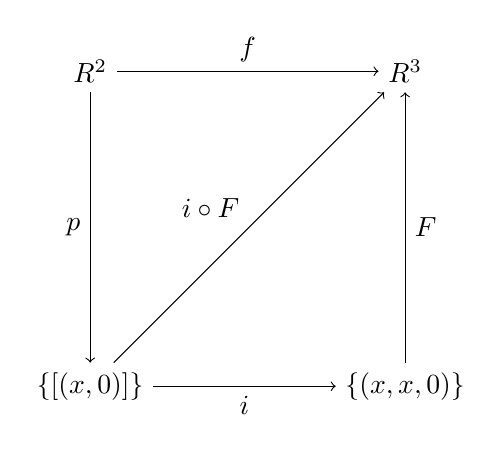
\begin{tikzpicture}
  \node (A) {$\mathbb{R}^2$};
  \node (B) [right of=A, node distance=4cm] {$\mathbb{R}^3$};
  \node (ker) [below of=A, node distance=4cm] {$\{[(x,0)]\}$};
  \node (Im) [right of=ker, node distance=4cm] {$\{(x,x,0)\}$};
  \path[->]  (A) edge [left] node {$p$} (ker)
            (A) edge [above] node {$f$} (B)
            (ker) edge [below] node {$i$} (Im)
            (Im) edge [right] node {$F$} (B)
            (ker) edge [above left] node {$i \circ F$} (B)
            ;
\end{tikzpicture}
\caption{$f(x,y) = (x,x,0)$ come composizione di due funzioni}
\end{figure}
\end{exmp}

\subsection{Teorema di omomorfismo per gli insiemi}
\begin{prop}
Per ogni $f : A \to B$ si ha $|Im_f| = |\ker f|$, ossia esiste una biezione $F : \ker f \to Im_f$.
\end{prop}
\begin{proof}
Per le definizioni di immagine di una funzione e nucleo di una funzione:
\[
Im_f = \{ b \in B : \exists \ a \in A \text{ t.c. } f(a) = b \}\subseteq B
\]
\[
\ker f = \{ [a] : \forall \ x \in [a] \ f(x) = f(a) \}
\]
$ \forall $ classe di $ \ker f \ F([a]) = f(a) = F([b]) \Rightarrow [a] = [b]$ e $\forall \ b \in Im_f \ b = f(a) \Rightarrow F([a]) = b$. $F$ \`e una funzione suriettiva e iniettiva, quindi gli elementi del $\ker f$ sono tanti quanti gli elementi di $Im_f$.
\end{proof}

\begin{figure}[ht]
\centering
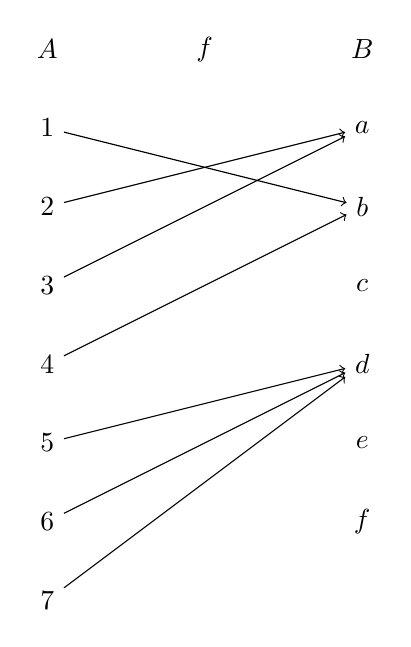
\begin{tikzpicture}
  \node (A) {$A$};
  \node (f) [right of=A, node distance=2cm] {$f$};
  \node (B) [right of=f, node distance=2cm] {$B$};
  \node (1) [below of=A, node distance=1cm] {$1$};
  \node (2) [below of=1, node distance=1cm] {$2$};
  \node (3) [below of=2, node distance=1cm] {$3$};
  \node (4) [below of=3, node distance=1cm] {$4$};
  \node (5) [below of=4, node distance=1cm] {$5$};
  \node (6) [below of=5, node distance=1cm] {$6$};
  \node (7) [below of=6, node distance=1cm] {$7$};
  \node (a) [below of=B, node distance=1cm] {$a$};
  \node (b) [below of=a, node distance=1cm] {$b$};
  \node (c) [below of=b, node distance=1cm] {$c$};
  \node (d) [below of=c, node distance=1cm] {$d$};
  \node (e) [below of=d, node distance=1cm] {$e$};
  \node (f) [below of=e, node distance=1cm] {$f$};
  \path[->]  (1) edge node {} (b)
            (2) edge node {} (a)
            (3) edge node {} (a)
            (4) edge node {} (b)
            (5) edge node {} (d)
            (6) edge node {} (d)
            (7) edge node {} (d)
            ;
\end{tikzpicture}
\caption{$\ker f = \{ [1], [2], [5]\}$, $Im_f = \{a, b, d\}$ }
\end{figure}

\subsubsection{Partizioni come reticoli}

$\Pi (A)$ \`e insieme delle partizioni di $A$, $\subseteq $ \`e una relazione di raffinamento.

Dati $\pi, \sigma \in \Pi(A)$, $\pi \subseteq \sigma \Leftrightarrow $ $\forall \ B \in \pi$ si ha che $B$ \`e contenuto in un blocco di $\sigma \Leftrightarrow $ ogni blocco di $\sigma$ \`e unione di blocchi di $\pi \Leftrightarrow \forall \ x, y \in A , \ x \ \varepsilon_{\pi} \ y \Rightarrow x \ \varepsilon_{\sigma} \ y$.

\begin{prop}
$\left( \Pi(A) , \subseteq \right)$ \`e un insieme parzialmente ordinato ed \`e un reticolo, ossia presi comunque due elementi c'\`e l'$\inf$ e il $\sup$.
\end{prop}
\begin{proof}
$(\pi \wedge \sigma)$ \`e dato dalla relazione $ x \ \varepsilon_{(\pi \wedge \sigma)} \ y \Leftrightarrow x \ \varepsilon_{\pi} \ y $ e $ x \ \varepsilon_{\sigma} \ y $. Quindi per definizione $\pi \wedge \sigma $ \`e $\inf( \pi, \sigma)$.
\end{proof}

Verifichiamone le propriet\`a:
\begin{itemize}
  \item $\pi \wedge \sigma \le \pi, \sigma$, vero per definizione di $\le$.
  \item $\pi \le \sigma \Leftrightarrow $ se $ x \ \varepsilon_{\pi} \ y $ allora $x \ \varepsilon_{\sigma} \ y$
  \item $\tau \le \pi, \sigma \Rightarrow \tau \le (\pi \wedge \sigma)$, infatti:
   \[
   x \ \varepsilon_{\tau} \ y \Rightarrow 
   x \ \varepsilon_{\pi} \ y \text{ e }
   x \ \varepsilon_{\sigma} \ y 
   \Rightarrow x \ \varepsilon_{(\pi \wedge \sigma)} \ y
   \]
\end{itemize}

\begin{defn}
$x \ \varepsilon_{(\pi \vee \sigma)} \ y \Leftrightarrow \exists \ x = a_1, a_2 \dots a_n = y $ tale che $a_i \ \varepsilon_{\pi} \ a_j$ oppure $a_i \ \varepsilon_{\sigma} \ a_j$ con $i \in [1, n-1]$, ossia ho una catena che mette in relazione $a_i$ con $a_j$ passando per $\pi$ o $\sigma$.
\end{defn}

Poich\'e $(\pi \vee \sigma) = \sup (\pi, \sigma)$, allora:
\begin{itemize}
  \item $\pi, \sigma \le (\pi \vee \sigma)$, ossia $\pi \le (\pi \vee \sigma)$ e $\sigma \le (\pi \vee \sigma)$, vero per definizione perch\'e $x \ \varepsilon_{\pi} \ y \Rightarrow x \ \varepsilon_{\pi \vee \sigma} \ y$.
  \item $\pi, \sigma \le \tau \Rightarrow (\pi \vee \sigma) \le \tau$, ossia $x \ \varepsilon_{\pi} \ y \Rightarrow x \ \varepsilon_{\tau} \ y$ e $x \ \varepsilon_{\sigma} \ y \Rightarrow x \ \varepsilon_{\tau} \ y$. Quando dico $x \ \varepsilon_{(\pi \vee \sigma)} \ y$, allora $x \ \varepsilon \ a_2 \ \varepsilon \dots \varepsilon \ y$, in cui ogni $\varepsilon$ \`e o $\varepsilon_{\pi}$ o $\varepsilon_{\sigma}$, quindi in ogni caso $a_i \ \varepsilon_{\pi} \ a_j$ o $a_i \ \varepsilon_{\sigma} \ a_j$ per cui necessariamente $a_i \ \varepsilon_{\tau} \ a_j$. Segue per transitivit\`a che $x \ \varepsilon_{\tau} \ y$.
\end{itemize}

\textbf{Esercizio:} $(\Pi(A), \subseteq)$ \`e un reticolo e $\subseteq$ \`e una relazione d'ordine. Dimostrare che non \`e modulare.
\vspace{5cm}

\section{Morfismi}

Sono delle funzioni $f : A \to B$ che partono da $A$ con una struttura e arrivano a $B$ con la stessa struttura.

\subsection{Morfismi di insiemi parzialmente ordinati}

Detti anche ``morfismi d'ordine'' o funzioni monotone. 
\begin{defn}
Un morfismo di un insieme parzialmente ordinato \`e un'applicazione $f : P_1 \to P_2$ dove $(P_1, \le_{1})$ e $(P_2, \le_{2})$ sono insiemi particolarmente ordinati, tale che $\forall \ x, y \in P_1$ con $x \le_1 y \Rightarrow f(x) \le_2 f(y)$. $f$ \`e una funzione monotona (ossia $f$ conserva l'ordine). 
\end{defn}
Quindi un morfismo va da un'insieme con una struttura ad un altro insieme con la sua struttura. Lo indicheremo con questa notazione:
\[
f : (P_1, \le_{1}) \to (P_2, \le_{2})
\]
\begin{exmp}
Dati $P_1 = P_2 = \mathbb{P}(\Gamma)$ e la relazione $(\mathbb{P}(\Gamma), \subseteq)$, definisco $f : \mathbb{P}(\Gamma) \to \mathbb{P}(\Gamma)$ come, fissato $A$ sottoinsieme finito di $\Gamma$, $\forall \ X \in \mathbb{P}(\Gamma) f(X) = A \cap X$.

$f$ \`e un morfismo $f : (\mathbb{P}(\Gamma), \subseteq) \to (\mathbb{P}(\Gamma), \subseteq)$ poich\'e $\forall \ X, Y \in \mathbb{P}(\Gamma) \ X \subseteq Y \Rightarrow f(X) \subseteq f(Y)$ visto che $X \cap A \subseteq Y \cap A$.
\end{exmp}
Questa propriet\`a si chiama \textbf{isotonia} di $\subseteq$. Anche l'unione ha questa propriet\`a: $g : (\mathbb{P}(\Gamma), \subseteq) \to (\mathbb{P}(\Gamma), \subseteq)$ con $g(X) = A \cup X$

\begin{exmp}
Sia $\Gamma$ un insieme finito, definisco una funzione su $\mathbb{P}(\Gamma)$ e $(\mathbb{N}, \le)$ $f : \mathbb{P}(\Gamma) \to \mathbb{N}$ come $\forall \ X \in \mathbb{P}(\Gamma) \ f(X) = |X|$. Anche questa \`e una funzione monotona.
\end{exmp}

\subsection{Morfismi di reticoli}

$(L, \le)$ \`e un reticolo se $\forall \ x, y \in L \ \exists \ \inf(x, y) $ e $ \exists \ \sup(x,y)$. Ogni reticolo individua una struttura algebrica con due operazioni, $(L, \wedge, \vee)$, e inoltre dalla struttura algebrica posso definire il reticolo.

\begin{defn}
Dati due reticoli $(L_1, \le_1)$ e $(L_2, \le_2)$, un morfismo di reticoli \`e una funzione $f : L_1 \to L_2$ che verifica le seguenti propriet\`a:
\begin{description}
  \item[M1\label{itm:M1}] $\forall \ x, y \in L_1 \ f(\inf(x,y)) = \inf(f(x),f(y))$, e analogamente $\forall \ x, y \in L_1 \ f(\sup(x,y)) = \sup(f(x),f(y))$.
  \item[M2\label{itm:M2}] Deve rispettare l'ordine. $\forall \ x, y \in L_1 $ con $x \le_1 y \Rightarrow f(x) \le_2 f(y)$.
\end{description}
\end{defn}

\begin{exmp}
Riprendendo l'esempio precedente, $P_1 = P_2 = \mathbb{P}(\Gamma)$ e la relazione $(\mathbb{P}(\Gamma), \subseteq)$, definisco $f : \mathbb{P}(\Gamma) \to \mathbb{P}(\Gamma)$ come, fissato $A$ sottoinsieme finito di $\Gamma$, $\forall \ X \in \mathbb{P}(\Gamma) \ f(X) = A \cap X$.

In questo reticolo, $\inf(X,Y) = X \cap Y$, quindi $f(\inf(X,Y)) = f(X \cap Y) = (X \cap Y) \cap A$. Per verificare \ref{itm:M1}, $(X \cap Y) \cap A = \inf(f(X,Y)) = \inf(X \cap A, Y \cap A) = (X \cap A) \cap (Y \cap A)$, vero per la propriet\`a commutativa, la propriet\`a associativa e l'idempotenza degli insiemi.
\[
(X \cap A) \cap (Y \cap A) = (X \cap A) \cap (A \cap Y) = X \cap (A \cap A) \cap Y = X \cap A \cap Y
\]
\end{exmp}

\begin{exmp}\label{morfismo_no_reticoli}
Sia $\Gamma$ un insieme finito, definisco una funzione su $\mathbb{P}(\Gamma)$ e $(\mathbb{N}, \le)$ $f : \mathbb{P}(\Gamma) \to \mathbb{N}$ come $\forall \ X \in \mathbb{P}(\Gamma) f(X) = |X|$.

Devo verificare \ref{itm:M1}. $f(\inf(X,Y)) = \inf(f(X),f(Y))$. $f(X \cap Y) = |X \cap Y|$, mentre $\inf(f(X),f(Y)) = \inf(|X|,|Y|)$, ossia il minore fra i due numeri. Non \`e vero in generale, quindi questa funzione non \`e un morfismo di reticoli.
\end{exmp}

In realt\`a \ref{itm:M1} implica \ref{itm:M2}, a differenza di quanto visto nelle relazioni di equivalenza e di ordine.

\begin{prop}
$(L, \le_1)$ e $(L, \le_2)$ due reticoli. Sia $f : L_1 \to L_2$ tale che $\forall \ x, y \in L_1 \ f(\inf(x,y)) = \inf (f(x),f(y))$ e $\forall \ x, y \in L_1 \ f(\sup(x,y)) = \sup (f(x),f(y))$, allora $f$ \`e una funzione monotona, e quindi \`e un morfismo di reticoli.
\end{prop}
\begin{proof}
Bisogna dimostrare che conserva l'ordine, ossia che se $x \le_1 y \Rightarrow f(x) \le_2 f(y)$. Per l'ipotesi, $\inf(x,y) = x$ e $\sup(x,y)= y$. Quindi $f(\inf(x,y)) = f(x)$. Per \ref{itm:M1} $f(\inf(x,y)) = \inf(f(x),f(y))$, quindi $f(x) = \inf(f(x),f(y)) \Rightarrow f(x) \le_2 f(y)$.
\end{proof}
Stessa dimostrazione vale per il $\sup$. Abbiamo dimostrato gi\`a che il contrario non vale, nell'esempio \ref{morfismo_no_reticoli}.

\subsection{Isomorfismi}
Un isomorfismo \`e un morfismo biunivoco.

Dato l'insieme delle parti di $\Gamma$, $(\mathbb{P}(\Gamma), \subseteq)$, e l'insieme $2 = \{ 0, 1 \}$, $2^{\Gamma}$ \`e l'insieme delle funzioni $\Gamma \to \{0,1\}$. Date due funzioni $f, g \in 2^{\Gamma}$, $f \le g \Leftrightarrow \forall \ x \in 2 $ ho che $ f(x) \le g(x)$ (come da  definizione \ref{ordine_funzioni}). 

$(2^{\Gamma}, \le)$ \`e un reticolo. Infatti $\inf(f,g) : \Gamma \to 2$ \`e:
\[
\inf(f,g)(x) = 
\begin{cases}
f(x) & \text{ se } f(x) \le g(y) \\
g(x) & \text{ altrimenti}
\end{cases}
\]
Analogamente, $\sup(f,g)(x) : \Gamma \to 2$ \`e:
\[
\sup(f,g)(x) = 
\begin{cases}
g(x) & \text{ se } f(x) \le g(y) \\
f(x) & \text{ altrimenti}
\end{cases}
\]

Un esempio di isomorfismo \`e quindi $F : \mathbb{P}(\Gamma) \to 2^{\Gamma}$. Prendo un sottoinsieme $A \subseteq \Gamma$ (ossia un elemento $A \in \mathbb{P}(\Gamma)$) e definisco la ``funzione caratteristica di $A$'' che indicher\`o con $\varphi_{A} : \Gamma \to 2$ che dice se un elemento di $\Gamma$ \`e o non \`e in $\Gamma$, ossia:
\[
\forall \ x \in \Gamma \ \varphi_A (x) = 
\begin{cases}
0 \text{ se } x \notin A \\
1 \text{ se } x \in A
\end{cases}
\]
$F$ \`e biunivoca. Dimostriamo che \`e iniettiva e suriettiva.
\begin{prop}
Se $A, B \in \mathbb{P}(\Gamma)$ e $\varphi_A = \varphi_B \Rightarrow A = B$, ossia per doppia inclusione $A \le B$ e $B \le A$.
\end{prop}
\begin{proof}
Per definizione di funzione caratteristica, $\forall \ x \in A \Rightarrow \varphi_A(x) = 1 = \varphi_B(x) \Rightarrow x \in B$.
\end{proof}
\begin{prop}
$\forall \ f \in 2^{\Gamma} \ \exists \ A \in \mathbb{P}(\Gamma)$ t.c. $\varphi_A = f$.
\end{prop}
\begin{proof}
Prendo $\Gamma = \{ 1, 2, 3, 4, 5, 6, 7\}$, e rappresento $f$ dal punto di vista dell'occupazione.

\begin{tabular}{ccccccc}
1 & 2 & 3 & 4 & 5 & 6 & 7 \\
0 & 0 & 1 & 1 & 0 & 1 & 0
\end{tabular}

Quindi $A = \{ 3, 4, 6 \} = f^{-1} (1)$, ossia la controimmagine di $\varphi_A$.
\end{proof}

Poich\'e $F$ \`e un isomorfismo, $A \subseteq B \Rightarrow F(A) \le F(B) = \varphi(A) \le \varphi(B)$, infatti $\forall \ x \in \Gamma$:
\[
\varphi_A(x) = 
\begin{cases}
0 \text{ se } x \notin A \Rightarrow \varphi_A(x) \le \varphi_B(x) \\
1 \text{ se } x \in A \Rightarrow \text{ poich\'e } A \subseteq B, \ \varphi_B(x) = 1 \Rightarrow \varphi_A(x) \le \varphi_B(X)
\end{cases}
\]
Dimostriamo che si tratta di un morfismo di reticoli.
\begin{prop}
$F(\inf(A,B)) = \inf(F(A), F(B))$, ossia $F(\inf(A,B)) = F(A \cap B) = \varphi_{(A \cap B)}$ e $\inf(F(A), F(B)) = \inf(\varphi_A, \varphi_B)$.

Quindi $\inf(\varphi_A, \varphi_B) = \varphi_{(A \cap B)}$.
\end{prop}
\begin{proof}
Per le propriet\`a dei reticoli:
\begin{itemize}
  \item $\varphi_{A \cap B} \le \varphi_A, \varphi_B$
  \[
  \forall \ x \in \Gamma \varphi_{A \cap B} (x) =
  \begin{cases}
  0 \text{ se } x \notin (A \cap B) \\
  1 \text{ altrimenti}
  \end{cases}
  \]
  \[
  \varphi_{A \cap B} (x) = 
  \begin{cases} 
  0 \le \varphi_A \\
  1 \Rightarrow x \in (A \cap B) \subseteq A \Rightarrow \varphi_A(x) = 1 \Rightarrow \varphi_{A \cap B} (x) \le \varphi_A (x)
  \end{cases}
  \]
  \item $f \le \varphi_A, \varphi_B \Rightarrow f \le \varphi_{A \cap B}$
  \begin{gather*}
  f \in 2^{\Gamma} \\
  f \le \varphi_A, \varphi_B \Rightarrow
  \forall \ x \in \Gamma \ f(x) \le 
  \varphi_A(x) 
  \text{ e } 
  \varphi_B(x) \\
  f(x) =
  \begin{cases}
  0 \le \varphi_{A \cap B} (x) \\
  1 \Rightarrow \varphi_A (x) = \varphi_B (x) = 1 \Rightarrow x \in (A \cap B) \Rightarrow \varphi_{A \cap B} (x) = 1
  \end{cases}
  \end{gather*}
\end{itemize}
\end{proof}

L'insieme delle parti di un insieme $\Gamma$ \`e in corrispondenza biunivoca con l'insieme delle funzioni da $\Gamma$ in 2, quindi hanno la stessa cardinalit\`a.

\subsubsection{Considerazioni generali sugli isomorfismi}

\begin{enumerate}
  \item Sia $F : (P, \le) \to (Q, \le)$ un isomorfismo da $P$ in $Q$, posso prendere la sua inversa $G : (Q, \le) \to (P, \le)$ che \`e a sua volta un isomorfismo da $Q$ in $P$.
  \item Se prendo tre strutture $P, G, R$ e due isomorfismi $F : (P, \le) \to (Q, \le)$ e $G : (Q, \le) \to (R, \le)$, $G \circ F : (P, \le) \to (R, \le)$.
  \item Le relazioni di equivalenza sono una generalizzazione dell'uguaglianza. La relazione di uguaglianza \`e la pi\`u piccola relazione di equivalenza, in cui tutte le classi sono costituite da un solo elemento.
  \item Se prendo tutte le possibili strutture d'ordine $(P, \le)$, posso creare una relazione di equivalenza per cui due strutture sono equivalenti se c'\`e un isomorfismo.

  Ossia, prendo due strutture $(P, \le)$ e $(Q, \le)$, e dico che $(P, \le)$ \`e equivalente a $(Q, \le)$ se esiste un isomorfismo da $P$ a $Q$. Lo indico con $(P, \le) \cong (Q, \le)$.
  \item Se due strutture sono isomorfe (come in figura \ref{fig:strutture_isomorfe}), posso studiare una sola struttura e le propriet\`a di quella struttura valgono su tutte le strutture isomorfe.
\end{enumerate}

\begin{figure}
\centering
\begin{tikzpicture}
  \node (6) {6};
  \node (5) [left of=6, node distance=1cm] {5};
  \node (4) [below right of=5, node distance=1cm] {4};
  \node (3) [below right of=4, node distance=1cm] {3};
  \node (2) [below of=4, node distance=1cm] {2};
  \node (1) [below of=2, node distance=1cm] {1};
  \path[-]  (6) edge node {} (4)
            (5) edge node {} (4)
            (4) edge node {} (2)
            (2) edge node {} (3)
            (1) edge node {} (2)
            ;
\end{tikzpicture}
\begin{tikzpicture}
  \node (6) {e};
  \node (5) [left of=6, node distance=1cm] {f};
  \node (4) [below right of=5, node distance=1cm] {d};
  \node (3) [below right of=4, node distance=1cm] {c};
  \node (2) [below of=4, node distance=1cm] {b};
  \node (1) [below of=2, node distance=1cm] {a};
  \path[-]  (6) edge node {} (4)
            (5) edge node {} (4)
            (4) edge node {} (2)
            (2) edge node {} (3)
            (1) edge node {} (2)
            ;
\end{tikzpicture}
\caption{\label{fig:strutture_isomorfe}Esempio di strutture isomorfe}
\end{figure}

\textbf{Esercizio:} trovare tutti i reticoli (a meno di isomorfismi) con 4 elementi.

\vspace{5cm}

\section{Numeri Naturali}

$\mathbb{N}$ \`e l'insieme dei numeri naturali. Seguiamo la definizione di Peano.
\begin{defn}[Numeri naturali]
L'insieme dei numeri naturali \`e un insieme non vuoto tale che:
\begin{description}
  \item[N1\label{itm:N1}] Esiste una funzione $\sigma : \mathbb{N} \to \mathbb{N}$ (una endofunzione) iniettiva detta ``successore'';
  \item[N2\label{itm:N2}] Esiste un elemento di $\mathbb{N}$ chiamato ``zero'' ed indicato con 0 tale che $0 \notin Im_{\sigma}$, ossia che non \`e il successore di nessun numero naturale;
  \item[N3\label{itm:N3}] Principio di induzione: se $U \subseteq \mathbb{N}$ tale che:
  \begin{itemize}
    \item $0 \in U$;
    \item $n \in U \Rightarrow \sigma(n) \in U$;
  \end{itemize}
  allora $U = \mathbb{N}$.
\end{description}
\end{defn}
Dire che un insieme \`e finito vuol dire che ogni iniezione sull'insieme \`e pure una suriezione. Quindi da \ref{itm:N1} e \ref{itm:N2} segue che $\mathbb{N}$ \`e infinito, poich\'e esiste una funzione iniettiva che non \`e suriettiva.
\begin{prop}
L'immagine di $\sigma$ \`e tutto $\mathbb{N}$ escluso lo 0. $Im_{\sigma} = \mathbb{N} \setminus \{ 0 \}$
\end{prop}
\begin{proof}
Sia $U = Im_{\sigma} \cup 0$. $U$ coincide con $\mathbb{N}$ per \ref{itm:N3}. Infatti:
\begin{itemize}
  \item $0 \in U$ per definizione di $U$;
  \item $\forall \ n \in U, \ \sigma(n) \in U$.
\end{itemize}
\end{proof}
L'elemento $\sigma(0)$ si indica con 1.

\subsection{Iterazioni}

Dato un insieme $A \neq \emptyset$ ed una funzione $f : A \to A$, con $\circ : A^A \times A^A \to A^A$ a indicare la composizione, $(A^A, \circ)$ \`e un monoide. Infatti $f \circ id_A = f = id_A \circ f$ \`e l'identit\`a.

\begin{defn}[Iterazioni]
Le iterazioni di $f : A \to A$ sono definite da:
\begin{itemize}
  \item $f^0 = id_A$;
  \item $\forall \ n \in \mathbb{N}$ definisco $f^{\sigma(n)} = f \circ f^n$.
\end{itemize}
\end{defn}
\begin{prop}
$f^n$ \`e ben definita per ogni $n \in \mathbb{N}$.
\end{prop}
\begin{proof}
Sia $U = \{ n \in \mathbb{N} : f^n $ \`e ben definita $\}$. $0 \in U$ per definizione. Se $n \in U f^n$ \`e definita, quindi \`e definita anche $f^{\sigma(n)} = f \circ f^n$, essendo $f$ data. Quindi $U = \mathbb{N}$.
\end{proof}
\subsubsection{Iterazioni di $\sigma$}
\begin{defn}
Definiamo le iterazioni di $\sigma$ come segue:
\begin{itemize}
  \item $\sigma^0 = id_{\mathbb{N}}$;
  \item $\sigma^{\sigma(n)} = \sigma \circ \sigma^n \ \forall \ n \in \mathbb{N}$.
\end{itemize}
\end{defn}

\begin{prop}\label{iterazione_nesima}
$\sigma^n(0) = n$
\end{prop}
\begin{proof}
Si dimostra per induzione. $U = \{ n \in \mathbb{N} : \sigma^n(0) = n \}$. 

Lo 0 \`e gi\`a $\in U$, poich\'e $\sigma^0 (0) = id_{\mathbb{N}}(0) = 0$.

$\sigma(n) \in U \Rightarrow \sigma^{\sigma(n)} (0) = \sigma(n)$. Per definizione delle iterazioni su $\sigma$, $\sigma^{\sigma(n)}(0) = \sigma \circ \sigma^{n} (0) = \sigma(n)$ poich\'e $\sigma(n) \in U$ per ipotesi.
\end{proof}

\begin{defn}[Potenze]
Ho un monoide $(M, \cdot)$. $\cdot : M \times M \to M $ associativa e con unit\`a $1_M$. $a \in M$ $a \cdot 1_M = a = 1_M \cdot a$
\begin{itemize}
  \item $a^0 = 1_M$
  \item $a^{\sigma(n)} = a \cdot a^n$
\end{itemize}
\textit{Sinceramente non ho capito che c'entra col resto e perch\'e sta qui.}
\end{defn}

\begin{prop}
$\forall \ n \in \mathbb{N} \setminus \{ 0 \}$, $0 \notin Im_{\sigma^n}$, ossia lo 0 non \`e nell'immagine di nessuna iterazione di $\sigma$, ossia comunque itero $\sigma$ non ottengo mai lo 0.
\end{prop}
\begin{proof}
Lo dimostriamo per assurdo. Supponiamo che $\exists \ n \in \mathbb{N}$ t.c. $0 \in Im_{\sigma^n} \Rightarrow \exists \ x \in \mathbb{N}$ t.c. $\sigma^n (x) = 0$. Poich\'e $n \neq 0 \Rightarrow n \in Im_{\sigma} = \mathbb{N} \setminus \{ 0 \} \Rightarrow n = \sigma(t)$. Quindi $0 = \sigma^n(x) = \sigma^{\sigma(t)}(x) = (\sigma \circ \sigma^t)(x) = \sigma(\sigma^t(x)) \Rightarrow 0 \in Im_{\sigma}$. Ho ottenuto l'assurdo con \ref{itm:N2}.
\end{proof}
Attraverso le tre propriet\`a che definiscono $\mathbb{N}$ si possono ritrovare tutte le altre propriet\`a di $\mathbb{N}$. 

\subsection{Operazioni su $\mathbb{N}$}

Possiamo definire il monoide $(\mathbb{N}, +)$. L'operazione di somma $+ : \mathbb{N} \times \mathbb{N} \to \mathbb{N}$ \`e definita cos\`i:
\[
m + n = \sigma^{n}(m)
\]
\textbf{Esercizio:} dimostare che \`e commutativa, e che quindi $\sigma^n(m) = \sigma^m(n)$. \vspace{5cm}

L'elemento neutro \`e lo 0, infatti: $ m + 0 = \sigma^0 (m) = id_{\mathbb{N}} (m) = m $ e $ 0 + m = \sigma^m (0) = m $ per la proposizione \ref{iterazione_nesima}.

\begin{oss}
$n + 1 = n + \sigma(0) = \sigma(n)$
\end{oss}

L'operazione + \`e associativa, oltre che commutativa. 

La somma in $\mathbb{N}$ ha la ``regola di cancellazione''. $\forall \ m, n, k \in \mathbb{N}$, se $m + k = n + k \Rightarrow m = n$. In realt\`a in $\mathbb{N}$ non esiste l'inverso, quindi questa regola ha poco a che vedere con la ``cancellazione''.

Tutte le propriet\`a sono pi\`u facili da dimostare con il seguente lemma.
\begin{lem}\label{successore_somma}
\[
m + \sigma (n) = \sigma(m + n)
\]
\end{lem}
\begin{proof}
\[
m + \sigma(n) = \sigma^{\sigma(n)} (m) = (\sigma \circ \sigma^n) (m) = \sigma ( \sigma^n (m) ) = \sigma(m + n)
\]
\end{proof}
\begin{defn}[Prodotto su $\mathbb{N}$]
$(\mathbb{N}, \cdot)$ \`e un'operazione $\cdot : \mathbb{N} \times \mathbb{N} \to \mathbb{N}$ tale che $\forall \ (m, n) \in \mathbb{N} \times \mathbb{N}$, $m \cdot n = (\sigma^m)^n(0)$.
\end{defn}
Il prodotto \`e un'operazione associativa e distributiva.

\begin{prop}
$\sigma(0) = 1$ \`e l'elemento neutro.
\end{prop}
\begin{proof}
$m \cdot \sigma(0) = (\sigma^m)^{\sigma(0)} (0) = \sigma^m (0) = m$

$\sigma(0) \cdot m = (\sigma^{\sigma(0)})^m (0) = \sigma^m (0) = m$
\end{proof}

\begin{defn}[Legge di annullamento del prodotto]
$m \cdot n = 0 \Leftrightarrow m = 0 $ oppure $ n = 0 $.
\end{defn}

Sul prodotto e sulla somma valgono le leggi distributive: $k \cdot (m+n) = k \cdot m + k \cdot n$ e, per commutativit\`a, $(m + n) \cdot k = m \cdot k + n \cdot k$.
\begin{lem}\label{prodotto_successore}
$m \cdot \sigma(n) = m \cdot n + m$
\end{lem}
\begin{proof}
$m \cdot \sigma(n)$ per definizione del prodotto \`e $ (\sigma^m)^{\sigma(n)} (0) $ che per definizione di iterazione \`e $ (\sigma^m \circ (\sigma^m)^n) (0) = \sigma^m ( (\sigma^m)^n (0)) = \sigma^m (m \cdot n) = m \cdot n + m$
\end{proof}
Usando i due lemmi (lemma \ref{successore_somma} e lemma \ref{prodotto_successore}) si ottengono tutte le propriet\`a delle operazioni su $\mathbb{N}$.

\subsection{Ordine naturale su $\mathbb{N}$}

Possiamo definire una relazione d'ordine totale (e naturale) su $\mathbb{N}$ usando le due operazioni.
\begin{defn}[Ordine naturale]
$m \le n \Leftrightarrow \exists \ k \in \mathbb{N} : m + k = n$
\end{defn}
\`E una relazione d'ordine totale (ossia l'insieme $\mathbb{N}$ \`e linearmente ordinato), ossia $\forall \ m, n \in \mathbb{N}$ si ha che $ m \le n$ oppure $n \le m$.

L'ordine naturale su $\mathbb{N}$ \`e un ``ordine buono'', ossia $(\mathbb{N}, \le)$ si dice ``bene ordinato''. Il ``buon ordinamento'' \`e equivalente all'assioma della scelta. Vuol dire che ogni suo sottoinsieme non vuoto ha un primo elemento. $\mathbb{R}$, ad esempio, non \`e bene ordinato.
\begin{proof}[Dimostrazione del buon ordinamento]
Dimostriamolo per assurdo. Suppongo esista un sottoinsieme $V \neq \emptyset$ che non ha un primo elemento. Ossia, $\forall \ v \in V \ \exists \ w \in V$ t.c. $w \le v$.

Consideriamo la proposizione $P_n$: ``$\forall \ n \in \mathbb{N} \land \ \forall \ v \in V, \ n \le v$'' e dimostriamo che \`e vera $\forall \ n \in \mathbb{N}$.

\`E vero con 0: $\forall \ v \in V 0 \le v$.

Supponiamo sia vero per un $n \in \mathbb{N}$, e dimostriamo che \`e vero per $\sigma(n) $ che $ \forall \ v \in V \sigma(n) \le v$.

Per ipotesi di induzione so che $\forall \ v \in V, \ n \le v \Rightarrow \exists \ x \in \mathbb{N}$ t.c. $n + x = v$, per la definizione di $\le$. $x$ non pu\`o essere 0, altrimenti $n$ sarebbe il primo elemento di $V$. Quindi $x \neq 0 \Rightarrow x = \sigma(y) = y + 1$, e quindi $n + y + 1 = v $ ma per la propriet\`a commutativa $n + 1 + y = v \Rightarrow \sigma(n) + y = v \Rightarrow \sigma(n) \le v$.

Siamo giunti all'assurdo. Se prendo $n = v + 1$ avrei che $v + 1 \le v$.
\end{proof}

\subsection{Altre forme del principio di induzione}

Se $n_0 \in U$ (base dell'induzione) e $n_0 \le n \in U \Rightarrow n+1 = \sigma(n) \in U$, quindi $U = \{ n \in \mathbb{N}, n_0  \le n\}$.

$\mathbb{Z} \simeq \mathbb{N} \times \mathbb{N} / \rho$ con $(m, n) \rho (p, q) \Leftrightarrow m + q = n + p$. Le classi di equivalenza sono $[(0,0)], [(m,0)]$ e $[(0,m)]$. Posso chiamarle anche 0, $m$ e $-m$

\section{Principi del calcolo combinatorio}

Enumerare corrisponde a mettere in fila una serie di elementi. Contare significa saper stabilire una corrispondenza biunivoca fra due insiemi, ossia saper dire che gli elementi di $A$ sono quanti gli elementi di $B$, e saper poi dire che l'insieme $A$ ha $n$ elementi, ossia ha tanti elementi quanti sono i primi $n$ numeri naturali, ossia tanti quanti gli elementi di $[n] = \{1, 2, \dots n \}$.

Dati due insiemi $A$ e $B$, se dico $A \rho B \Leftrightarrow $ esiste una corrispondenza biunivoca da $A$ a $B$, verifico che $\rho$ \`e:
\begin{itemize}
   \item riflessiva;
   \item simmetrica;
   \item transitiva.
 \end{itemize} 
 Quindi $\rho$ \`e una relazione di equivalenza nell'insieme degli insiemi finiti. $A \rho B \Leftrightarrow |A| = |B| \Leftrightarrow A \leftrightarrow B \Leftrightarrow$ la cardinalit\`a di $A$ \`e uguale alla cardinalit\`a di $B$.

\subsection{Principio della somma}

\begin{prop}[Principio della somma]
 Dati $A$, $B$ tali che $A \cap B = \emptyset$, segue che $|A \cup B| = |A| + |B|$.
\end{prop}
\begin{proof}
$|A| = m$, $|B| = n$. Devo quindi poter realizzare una corrispondenza biunivoca $F$ fra $|A \cup B|$ e $[m + n]$. Ossia, dati $A = \{ a_1, a_2, \dots a_m\}$ e $B = \{ b_1, b_2 \dots b_n\}$, ho che $F(a_i) = i$ e $F(b_i) = m + i$.
\end{proof}

\`E possibile generalizzare la regola della somma.
\begin{prop}[Principio della somma 2]
Dati $t$ insiemi $A_1, \dots A_t$ tali che $A_i \cap A_j = \emptyset$ se $i \neq j$, ho che:
\[
\left| \bigcup_{i = 1}^{t} A_i\right| = \sum_{i = 1}^{t} |A_i|
\]
\end{prop}

$+ \mapsto A \dotcup B$ con $ A \cap B = \emptyset$.

\subsection{Principio del prodotto}

\begin{prop}[Principio del prodotto]
Dati $A$, $B$, ho che $|A \times B| = |A| \cdot |B|$.
\end{prop}
\begin{proof}
C'\`e una corrispondenza biunivoca $F : (A \times B) \to [m \cdot n]$. Quanto vale $F (a_i, b_j)$? In generale, contando con il metodo della diagonale (figura \ref{fig:metodo_diagonale}), ho che sulla diagonale $k$-esima trovo tutte le coppie tali per cui $i + j = k + 1$.

\begin{figure}
\centering
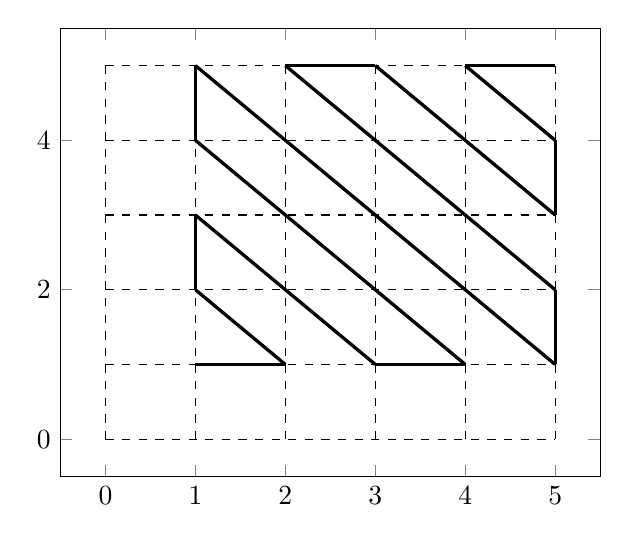
\begin{tikzpicture}
\begin{axis}[
    % graph options
]
\addplot[dashed,-] coordinates {(0,0) (0,5)};
\addplot[dashed,-] coordinates {(1,0) (1,5)};
\addplot[dashed,-] coordinates {(2,0) (2,5)};
\addplot[dashed,-] coordinates {(3,0) (3,5)};
\addplot[dashed,-] coordinates {(4,0) (4,5)};
\addplot[dashed,-] coordinates {(5,0) (5,5)};
\addplot[dashed,-] coordinates {(0,0) (5,0)};
\addplot[dashed,-] coordinates {(0,1) (5,1)};
\addplot[dashed,-] coordinates {(0,2) (5,2)};
\addplot[dashed,-] coordinates {(0,3) (5,3)};
\addplot[dashed,-] coordinates {(0,4) (5,4)};
\addplot[dashed,-] coordinates {(0,5) (5,5)};
\addplot[very thick, -] coordinates {(1,1) (2,1)};
\addplot[very thick, -] coordinates {(2,1) (1,2)};
\addplot[very thick, -] coordinates {(1,2) (1,3)};
\addplot[very thick, -] coordinates {(1,3) (3,1)};
\addplot[very thick, -] coordinates {(3,1) (4,1)};
\addplot[very thick, -] coordinates {(4,1) (1,4)};
\addplot[very thick, -] coordinates {(1,4) (1,5)};
\addplot[very thick, -] coordinates {(1,5) (5,1)};
\addplot[very thick, -] coordinates {(5,1) (5,2)};
\addplot[very thick, -] coordinates {(5,2) (2,5)};
\addplot[very thick, -] coordinates {(2,5) (3,5)};
\addplot[very thick, -] coordinates {(3,5) (5,3)};
\addplot[very thick, -] coordinates {(5,3) (5,4)};
\addplot[very thick, -] coordinates {(5,4) (4,5)};
\addplot[very thick, -] coordinates {(4,5) (5,5)};
\end{axis}
\end{tikzpicture}
\caption{\label{fig:metodo_diagonale}Metodo della diagonale}
\end{figure}
\end{proof}

\`E possibile generalizzare la regola del prodotto.
\begin{prop}[Principio del prodotto 2]
Se prendo un insieme finito di insiemi $A_1, \dots a_t$, ho che:
\[
\left| A_1 \times \dots \times A_t \right| = |A_1| \cdot \ldots \cdot |A_t|
\]
\end{prop}
\begin{proof}
Si dimostra per induzione su $t$.
\end{proof}

\begin{defn}[Principio del prodotto 3]
Dato un sottoinsieme $S$ del prodotto cartesiano $X^n$, $S \subseteq X^n$, ossia un insieme di $n$-uple, se verifico che:
\begin{itemize}
  \item al primo posto di una $n$-upla in $S$ ci sono $i_1$ elementi;
  \item $\forall \ j = 2 \dots n-1$ ci sono $i_j$ $n$-uple che hanno le prime $j-1$ coordinate uguali;
\end{itemize}
allora $|S| = i_1 \cdot i_2 \cdot \dots i_n$.
\end{defn}

\subsection{Dimostrazioni biettive}

Se voglio dimostrare che $a = b$, posso trovare due insiemi $A$ e $B$ tali che $|A| = a$ e $|B| = b$, e dimostrare che sono in biezione. Si indica solitamente con $A \leftrightarrow B$.

Due insiemi con intersezione disgiunta possono essere i due blocchi di una partizione con due soli blocchi.

\begin{prop}
Dato l'insieme delle funzioni da $A$ in $R$ $R^A = \{ f : A \to R\}$, se $|A| = n$ e $|R| = r$, allora $|R^A| = r^n = |R^n|$. Quindi esiste una biezione fra $R^A$ e $R^n$. $R^n$ \`e il prodotto di $R$ con s\'e stesso $n$ volte. Quindi le funzioni da $A$ in $R$ sono quante le $R$-uple di $n$ elementi.
\end{prop}
\begin{proof}
Data una funzione $f : A \to R$, definisco $F : R^A \to R^n$ tale che $(f, A = \{ a_1, \dots a_n\}) \mapsto (f(a_1), \dots f(a_n))$, che dal punto di vista dell'occupazione \`e:

\begin{tabular}{cccc}
$a_1$ & $a_2$ & $\dots$ & $a_n$ \\
$f(a_1)$ & $f(a_2)$ & $\dots$ & $f(a_n)$ 
\end{tabular}

Ossia, ad ogni funzione $f : A \to R$ associo la $n$-upla dei valori di $f$ ordinata seguendo un ordine lineare degli elementi di $A$.
\end{proof}
\begin{prop}
Dati $A, B$ disgiunti, $R^A \times R^B$ ha cardinalit\`a $|R^A \times R^B| = |R^{A \cup B}|$, dato che $|R^A| = r^n$ e $|R^B| = r^m$ e che quindi $r^n \cdot r^m = r^{n + m}$.

Quindi $|R^A \times R^B| $ e $ |R^{A \cup B}|$ sono in corrispondenza biunivoca.
\end{prop}
\begin{proof}
Esiste una biezione $F : R^A \times R^B \to R^{A \cup B}$. Questa funzione prende una coppia di funzioni e ne restituisce una terza $(f : A \to R, g: B \to R) \mapsto h : (A \cup B) \to R$ definita come, $\forall \ x \in A \cup B$:
\[
h(x) = 
\begin{cases}
f(x) \text{ se } x \in A\\
g(x) \text{ se } x \in B
\end{cases}
\]
\end{proof}
Dati due insiemi $R$, $S$ ed un insieme $A$:
\[
|R^A \times S^A| = |(R \times S)^A|
\]
\[
|(R^A)^B| = |R^{A \cdot B}|
\]
\textbf{Esercizio:} definire la biezione che dimostra le due propriet\`a precedenti.
\vspace{5cm}

La maggior parte dei numeri positivi che compaiono in combinatoria hanno un'interpretazione in teoria degli insiemi.

\subsection{Fattoriale decrescente}

\begin{defn}
Il fattoriale decrescente \`e una successione:
\begin{equation}
\{[r]_n\}_{n \in \mathbb{N}} \text{ : }
\begin{cases}
[r]_0 = 1 \\
[r]_{n+1} = [r]_n \cdot (r - n)
\end{cases}
\end{equation}
\end{defn}
\`E evidente che:
\[
[r]_n = \frac{r!}{(r-n)!}
\]

\begin{oss}
$[r]_n = 0$ se $r < n$. Inoltre, $[r]_n = n!$ se $r = n$.
\end{oss}

\begin{prop}
Dato $In(A,R)$, l'insieme delle funzioni iniettive da $A$ in $R$, se $|A| = n$ e $|R| = r$, allora $|In (A,R)| = [r]_n$.

In altre parole, il fattoriale decrescente $[r]_n$ corrisponde all'insieme delle funzioni iniettive da $A$ in $R$ $In(A,R)$.

\[
\left| In(A,R) \right| = \left| In (A- \{x\},R) \right| \cdot \left| R - Im_f \right|
\]

\end{prop}
\begin{proof}
Ricordiamo la definizione di iniettivit\`a: $\forall \ x, y \in A$ se $f(x) = f(y) \Rightarrow x = y$, $f$ \`e iniettiva.

Dimostriamo ora la proposizione per induzione. Se $A = \emptyset$, $|In(\emptyset, R)| = 1$.

Supponendo di aver calcolato il numero di funzioni inettive da un insieme con $n$ elementi ad un insieme con $r$ elementi (ossia $[r]_n$), dobbiamo determinare $[r]_{n+1}$.

Se $|A| = (n+1)$, sapendo che tutti gli elementi di $A$ sono distinti, prendo $x \in A$.

Data una funzione $f : A \to R$, questa individua una coppia $(f(x), f^{-} : A \setminus \{ x \} \to R)$ dove $f^{-}$ \`e definita come $f$ ossia $f^{-} (a) = f(a)$.

In quanti modi si pu\`o scegliere $f(x)$? In $|R \setminus Im_{f^-}|$ modi (ossia, $r - n$). Le funzioni iniettive da $A \setminus \{ x \}$ in $R$ sono $[r]_n$ per definizione, quindi per il principio del prodotto il numero di coppie che posso creare sono $[r]_{n+1} = [r]_n \cdot (r - n)$.
\end{proof}

\begin{prop}
Sappiamo che $|\mathbb{P}(A)| = |2^A| = 2^n$ con $|A| = n$. Quanti sono i sottoinsiemi pari di $A$, ossia $S \subseteq A $ t.c. $|S| = 2k$?

Gli insiemi di cardinalit\`a pari sono tanti quanti quelli di cardinalit\`a dispari, quindi sono $2^{n-1}$.
\end{prop}
\begin{proof}
So che $2^{n-1} = |\mathbb{P}(A \setminus \{x\})|$, quindi l'insieme dei sottoinsiemi pari di $A$ \`e in biezione con l'insieme delle parti di $A$ a cui ho tolto un elemento. Indicando con $P$ l'insieme dei sottoinsiemi pari di $A$, ho una biezione $F : \mathbb{P}(A \setminus \{x\}) \to P$:
\[
F(S) = 
\begin{cases}
S \text{ se } S \text{ \`e pari} \\
S \cup \{ x \} \text{ se } S \text{ \`e dispari} \\
\end{cases}
\]
\end{proof}

\subsection{Coefficienti  binomiali}
Indichiamo con $\binom{n}{k}$ il numero di sottoinsiemi con $k$ elementi di un insieme con $n$ elementi. Vediamo subito che $\binom{n}{k}$ per $k > n$ \`e 0. $\binom{n}{0} = 1$, $\binom{n}{1} = n$. Inoltre $\binom{n}{k} = \binom{n}{n-k}$, ossia il numero di sottoinsiemi con $k$ elementi \`e uguale al numero dei loro insiemi complementari.
\begin{prop}[Definizione ricorsiva di Pascal dei coefficienti binomiali]
\begin{equation}
\binom{n}{k} = \binom{n-1}{k} + \binom{n-1}{k-1}
\end{equation}
$\binom{n}{k}$ \`e il numero di sottoinsiemi con $k$ elementi, indicato con $\mathbb{P}_{k}(A)$. Lo divido in due sottoinsiemi disgiunti, con cardinalit\`a rispettivamente $\binom{n-1}{k}$ e $\binom{n-1}{k-1}$.

Fissato un $x \in A$, $\binom{n-1}{k}$ \`e l'insieme di tutti i sottoinsiemi con $k$ elementi di $A \setminus \{ x \}$, $\binom{n-1}{k-1}$ \`e l'insieme di tutti i sottoinsiemi con $k - 1$ elementi di $A \setminus \{x \}$.
\end{prop}
\begin{proof}
$\forall \ S \subseteq A$ con $|S| = k$ e $x \in A$ ho due casi: $x \in S$ o $x \notin S$. Definisco la biezione $F : \mathbb{P}_k (A) \to \mathbb{P}_k (A \setminus \{ x \}) \cup \mathbb{P}_{k - 1} (A \setminus \{ x \})$ come:
\[
F (S) =
\begin{cases}
S \text{ se } x \notin S \\
S \setminus \{ x \} \text{ se } x \in S
\end{cases}
\]
Ho quindi che $\mathbb{P}_k (A) = X \cup Y$ con $X = \{ S \subseteq A : |S| = k \land x \in S \}$ e $Y = \{ S \subseteq A : |S| = k \land x \notin S\}$. Se tolgo $x$ da $A$, le cardinalit\`a dei due insiemi diventano $|X| = \binom{n - 1}{k - 1}$ e $|Y| = \binom{n - 1}{k}$.
\end{proof}

% TODO che vuol dire questo
% $\{ r^n \}_{n \in \mathbb{N}} \leftrightarrow \{ f : A_n \to R\} = \{ |R^{A_n}| \}$ con $|A_n| = n$ e $|R| = r$.

\begin{prop}
Quanto valgono i coefficienti binomiali? Diciamo questo:
\[
[r]_n = n! \cdot \binom{r}{n}
\]
da cui segue che:
\[
\binom{r}{n} = \frac{[r]_n}{n!} = \frac{r!}{n! \cdot {r-n}!}
\]
Stiamo dicendo quindi che $[r]_n$ (il numero di funzioni iniettive da $A$ in $R$ con $|A| = n$ e $|R| = r$) \`e uguale alla cardinalit\`a di un insieme di coppie $|E|$. $n!$ \`e il numero di elementi al secondo posto della coppia, $\binom{r}{n}$ \`e il numero di elementi al primo posto.
\end{prop}
\begin{proof}
$\binom{r}{n}$ \`e il numero di sottoinsiemi con $n$ elementi di un insieme con $r$ elementi.
\[
E = \{ (S, ?) \text{ con } |S| = n \land S \subseteq R \}
\]
Abbiamo visto che ogni funzione $f : A \to R$ individua un'insieme immagine $Im_f \subseteq R$ e una partizione $\ker f \in \Pi(A)$, e che questi due insiemi sono in corrispondenza biunivoca $|Im_f| = |\ker f |$.

Se prendo una funzione iniettiva, il nucleo della funzione \`e la partizione pi\`u piccola, avendo per elementi le classi rappresentate dai singoli elementi del dominio. Quante sono le iniezioni $In(A, S)$ con $S = Im_f$? $[n]_n = n!$

Quindi, $ E = \{ (S, \bar f : A \to S) $, con $ |S| = n \land S \subseteq R $ e $\bar f : A \to S$ insieme delle biezioni da $A$ in $S$ $\}$
\end{proof}

\subsection{Teorema binomiale}
\begin{prop}[Teorema binomiale\label{teorema_binomiale}]
\[
\forall \ n \in \mathbb{N} \text{ con } n > 0 \ 
(x + y)^n = 
\sum_{k = 0}^n \binom{n}{k} \ x^k y^{n - k}
\]
\end{prop}
Si possono dimostrare anche identit\`a polinomiali con le biezioni. Quando sono uguali due polinomi? Quando nel loro sviluppo hanno tutti i coefficienti uguali.
\begin{theorem}[Identit\`a polinomiale]
Dati due polinomi in $n$ variabili $p(x_1, \ \dots \ x_n)$ e $q(x_1, \ \dots \ x_n)$, sono uguali se coincidono su insiemi infiniti, ossia se $\forall \ (a_1, \ \dots \ a_n) \in I^n$ con $I \subseteq \mathbb{R} $ e $ |I| = \infty$, $p(a_1, \ \dots \ a_n) = q(a_1, \ \dots \ a_n)$, ossia i due polinomi coincidono ($p = q$).
\end{theorem}
Al posto di $x$ e di $y$ posso quindi mettere due interi $r, s \in \mathbb{N}$, e dimostrare che $(r + s)^n = \sum_{k = 0}^n \binom{n}{k} r^k s^{n - k}$.
\begin{proof}
Il membro sinistro della proposizione equivalente alla definizione \ref{teorema_binomiale}, $(r + s)^n$, \`e la cardinalit\`a dell'insieme di funzioni da un insieme con $n$ elementi ad uno con cardinalit\`a $r + s$, ossia all'unione disgiunta di due insiemi con cardinalit\`a rispettivamente $r$ e $s$. Dicendo quindi che gli insiemi $A$, $R$ e $S$ hanno cardinalit\`a $|A| = n$, $|R| = r $ e $|S| = s$, e che $T = R \cup S$, ho che $(r + s)^n = \left| T^A \right|$.

Il membro destro della proposizione \`e una somma, quindi corrisponde all'unione disgiunta di $n$ insiemi.
\[
\left| \bigsqcup_{k = 0}^{n} E_k \right| = \sum_{k = 0}^{n} \left| E_k \right|
\text{ con }
|E_k| = \binom{n}{k} \ r^k s^{n - k}
\]
Devo definire l'insieme $E_k$. Per il principio del prodotto, \`e una terna:
\[
\left( X, \ f_k : X \to R, \ g_{(n - k)} : (A \setminus X) \to S \right)
\]
con $X \subseteq A$ tale che $|X| = k$, $f_k$ appartenente all'insieme delle funzioni da $X$ in $R$, e $g_{(n-k)}$ appartenente all'insieme delle funzioni da $A \setminus X$ (ossia il complementare di $X$) in $S$.

Dobbiamo mostrare ora che $T^A \leftrightarrow \bigsqcup E_k$, ossia che c'\`e una biezione. La funzione biettiva $F$ associa ad una funzione $f : A \to T$ una terna:
\[
\left( f^{-1} (R), \ f_k : X \to R, \ g_{(n - k)} : (A \setminus X) \to S \right) \in E_k
\]
con $f^{-1}(R) = X$ a indicare la controimmagine di $R$ e $|f^{-1}(R)| = k$.
\end{proof}

\subsection{Coefficienti multinomiali}

Il coefficiente multinomiale, indicato con:
\[
\binom{n}{k_1 \dots k_t}
\]
\`e il numero delle $t$-scomposizioni di un insieme $A$ con $n$ elementi nella forma $(E_1, \dots, E_t)$ tali che $|E_1| = k_1, \dots |E_t| = k_t$.

\begin{defn}[$t$-scomposizioni]
Sia $A$ un insieme con $n$ elementi, una $t$-scomposizione di $A$ \`e una $t$-upla $(E_1, \dots E_t)$ tale che:
\begin{description}
  \item[1S] $\bigsqcup_{i = 1}^{t} E_i = A$
  \item[2S] $E_i \cap E_j = \emptyset$ se $i \neq j$ 
\end{description}
$E_i$ \`e detto blocco.
\end{defn}
Ci sono due differenze fra una $t$-scomposizione e una partizione.
\begin{itemize}
  \item Un blocco di una scomposizione pu\`o anche essere vuoto, un blocco di una partizione \`e necessariamente $\neq \emptyset$.
  \item Considero un insieme $A = \{ a, b, c, d, e, f, g\}$. Posso avere una partizione:
  \[
  \pi = \{ \{a\}, \{b, g, f\}, \{c, d\}, \{e\} \}
  \]
  e due 4-scomposizioni distinte:
  \[
  (\{a\}, \{b, g, f\}, \{c, d\}, \{e\}) \neq 
  (\{a\}, \{c, d\}, \{b, g, f\}, \{e\})
  \]
  poich\'e le $t$-scomposizioni sono ordinate.
\end{itemize} 

Il coefficiente multinomiale \`e una generalizzazione del coefficiente binomiale.
\[
\binom{n}{k} = \binom{n}{k, n-k}
\]
Partendo da questa uguaglianza, so che:
\[
\binom{n}{k} = \binom{n}{k, n-k} = \frac{n!}{k! \ (n - k)!}
\Rightarrow
\binom{n}{k_1, \dots k_t} = \frac{n!}{k_1! \ \dots \ k_t!}
\]

\begin{prop}\label{coeff_mult_valore}
Il numero delle $t$-scomposizioni di $A$ $(E_1, \dots E_t)$ di $A$ (indicato anche con $E_1 + \dots + E_t = A$) tali che $|E_1| = k_1, \dots |E_t| = k_t$ \`e:
\begin{equation}
\binom{n}{k_1, \dots k_t} = \frac{n!}{k_1! \ \dots \ k_t!}
\end{equation}
\end{prop}
\begin{proof}
Per $t = 2$ \`e vero. Supponiamo sia vero per $t > 2$. Prendiamo una $(t+1)$-scomposizione $(E_1, \dots, E_t, E_{t+1})$ di $A$. Ogni scomposizione individua una coppia:
\[
\left( E_{t+1}, (E_1, \dots E_t) \right)
\]
in cui $E_{t+1} \subseteq A$ e $(E_1, \dots E_t)$ \`e una $t$-scomposizione di $A \setminus E_{t+1}$, poich\'e $E_1 + \dots + E_t + E_{t+1} = A$.

In quanti modi posso scegliere un sottoinsieme $|E_{t+1}| = k_{t+1}$? In $\binom{n}{k_{t+1}}$ modi. Quindi quante coppie $(E_{t+1}, (E_1, \dots E_t))$ ho? \`E un prodotto, e per il principio del prodotto:
\[
\binom{n}{k_{t+1}} \cdot \frac{(n - k_{t+1})!}{k_1! \dots k_{t}!}
\]
Semplificando, si ottiene la tesi.
\end{proof}

\subsection{Teorema multinomiale}
\begin{prop}
\begin{equation}
(x_1 + \dots + x_t)^n = \sum_{(k_1, \dots k_t) | k_1 + \dots k_t = n}
\binom{n}{k_1, \dots, k_t} \ x_1^{k_1} \dots x_t^{k_t}
\end{equation}
Dove la sommatoria indica la somma di tutte le $t$-uple $(k_1, \dots k_t)$ tali che $k_1 + \dots + k_t = n$.
\end{prop}
\begin{proof}
Si dimostra di nuovo per biezione. Prendo $x_i = r_i \in \mathbb{N}$. Quindi:
\[
(r_1 + \dots + r_t)^n = \sum_{(k_1, \dots k_t) | k_1 + \dots k_t = n}
\binom{n}{k_1, \dots, k_t} \ r_1^{k_1} \dots r_t^{k_t}
\]
Il membro sinistro \`e uguale alla cardinalit\`a dell'insieme delle funzioni da $A$ in $T$ tali che $T = R_1 \cup \dots \cup R_t$, in cui $R_i $ con $i \in [1, t]$ sono insiemi a due a due disgiunti tali che $| R_i | = r_i$.

Ogni funzione individua una scomposizione di $A$ in $t$-blocchi, in cui ogni blocco \`e dato dalla controimmagine $f^{-1} (R_i)$ ed ha cardinalit\`a $k_i$. 

Il membro destro \`e dato quindi dall'unione disgiunta di una serie di insiemi di $(t+1)$-tuple. Ciascuna $(t+1)$-upla ha al primo posto una $t$-scomposizione di $A$, e all'$(i+1)$-esimo posto una funzione dal blocco $K_i$ nell'insieme $R_i$. Per il principio del prodotto, il numero di queste $(t+1)$-uple, per ogni possibile $t$-scomposizione, \`e proprio:
\[
\binom{n}{k_1, \dots, k_t} \ r_1^{k_1} \dots r_t^{k_t}
\]
Come nel caso del teorema binomiale, per dimostrare la biezione basta definire la funzione biettiva $F : T^A \to$ l'insieme di queste $(t+1)$-uple, che a ciascuna funzione $f : A \to T$ associa la $t$-scomposizione di $A$ in cui ogni blocco \`e definito dalla controimmagine $f^{-1} (R_i)$ e tutte $t$ funzioni che da un blocco $K_i$ vanno in $R_i$.
\end{proof}

\begin{cor}[Corollario del teorema multinomiale\label{corollario_multinomiale}]
\[
\sum_{k = 0}^{n} (-1)^k \binom{n}{k} = 0
\]
\end{cor}
\begin{proof}
\[
(x - 1)^n = \sum_{k = 0}^{n} \binom{n}{k} (-1)^k x^{n-k}
\]
Ponendo $x = 1$, per il teorema binomiale, ho la tesi.
\end{proof}

\subsection{Principio dei cassetti}

$R^A$ \`e l'insieme delle funzioni da $A$ in $R$. $|R^A| = r^n$. Una funzione $f : A \to R \in R^A$ la posso interpretare in due modi:
\begin{description}
  \item[Punto di vista dell'occupazione] $A$ viene interpretato come un insieme di oggetti. Il codominio $R$ viene interpretato come un insieme di cassetti. Quindi una funzione da $A$ in $R$ \`e un modo di disporre gli oggetti di $A$ nei cassetti di $R$.
  \item[Punto di vista della distribuzione] Rappresento l'insieme $A$ come un insieme di posti, e l'insieme $R$ come un insieme di lettere (ossia come un alfabeto). Una funzione $f : A \to R$ mi d\`a una parola, ossia un modo di disporre le lettere di $R$ nei posti di $A$.
\end{description}
\begin{prop}[Principio dei cassetti]
Se $|A| > |R|$ non esistono funzioni iniettive da $A$ in $R$.
\end{prop}
Dal punto di vista dell'occupazione, se si mettono $|A| = n$ oggetti in $|R| = r$ cassetti con $n > r$, allora almeno un cassetto conterr\`a pi\`u di un oggetto. 

Dal punto di vista della distribuzione, ogni parola di lunghezza $n$ con lettere in un alfabeto di cardinalit\`a $r$, con $n > r$, contiene almeno una lettera ripetuta.

I due punti di vista hanno una formalizzazione matematica distinta.

\begin{prop}
Dato un triangolo equilatero di lato 1, e dati 5 punti interni, almeno 2 di essi hanno distanza minore di $\frac{1}{2}$.
\end{prop}
\begin{proof}
Si pu\`o partizionare il triangolo in 4 blocchi come in figura \ref{fig:triforza}, in modo che dati due punti qualsiasi in uno stesso blocco questi siano a meno di $\frac{1}{2}$ di distanza.
\begin{figure}[ht]
\centering
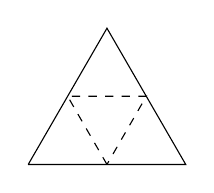
\begin{tikzpicture}
\draw (0,0) -- (2,0) -- (1,1.73)-- (0,0);
\draw[dashed] (1,0) -- (0.5,0.866) -- (1.5,0.866) -- (1,0);
\end{tikzpicture}
\caption{\label{fig:triforza}Le quattro partizioni possibili}
\end{figure}
\end{proof}

\begin{prop}
Se si colorano i punti del piano con due colori (R,B) esisterà un rettangolo con tutti i vertici dello stesso colore.
\end{prop}
\begin{proof}
Se prendo tre punti allineati, so che almeno due hanno lo stesso colore. Se prendo nove terne di punti allineati, a loro volta allineate in modo da poter formare un rettangolo con ciascuna coppia di terne, so che almeno due terne hanno la stessa combinazione di colori (figura \ref{fig:piano_punti_colore}).
\begin{figure}[ht]
\centering
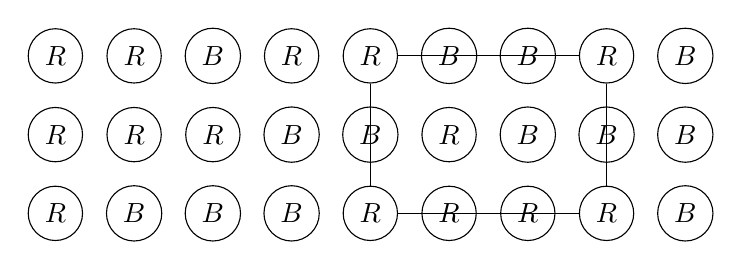
\begin{tikzpicture}
  \node (11) [circle, draw] {$R$};
  \node (12) [below of=11, circle, draw] {$R$};
  \node (13) [below of=12, circle, draw] {$R$};

  \node (21) [right of=11, circle, draw] {$R$};
  \node (22) [below of=21, circle, draw] {$R$};
  \node (23) [below of=22, circle, draw] {$B$};

  \node (31) [right of=21, circle, draw] {$B$};
  \node (32) [below of=31, circle, draw] {$R$};
  \node (33) [below of=32, circle, draw] {$B$};

  \node (41) [right of=31, circle, draw] {$R$};
  \node (42) [below of=41, circle, draw] {$B$};
  \node (43) [below of=42, circle, draw] {$B$};

  \node (51) [right of=41, circle, draw] {$R$};
  \node (52) [below of=51, circle, draw] {$B$};
  \node (53) [below of=52, circle, draw] {$R$};

  \node (61) [right of=51, circle, draw] {$B$};
  \node (62) [below of=61, circle, draw] {$R$};
  \node (63) [below of=62, circle, draw] {$R$};

  \node (71) [right of=61, circle, draw] {$B$};
  \node (72) [below of=71, circle, draw] {$B$};
  \node (73) [below of=72, circle, draw] {$R$};

  \node (81) [right of=71, circle, draw] {$R$};
  \node (82) [below of=81, circle, draw] {$B$};
  \node (83) [below of=82, circle, draw] {$R$};

  \node (91) [right of=81, circle, draw] {$B$};
  \node (92) [below of=91, circle, draw] {$B$};
  \node (93) [below of=92, circle, draw] {$B$};

  \draw (51) -- (81);
  \draw (81) -- (83);
  \draw (83) -- (53);
  \draw (53) -- (51);
\end{tikzpicture}
\caption{\label{fig:piano_punti_colore}Il rettangolo realizzabile sul piano colorato}
\end{figure}
\end{proof}
Prendo l'insieme $I = \{ 0, 1, 2 \}$ e definisco $X = I \times I \times I$. Definisco la relazione di equivalenza $\rho$ come:
\[
(x, y, z) \ \rho \ (x', y', z') \Leftrightarrow \{ x, y, z \} = \{ x', y', z'\}
\]
$\rho$ divide $X$ in classi di equivalenza. Quali sono gli elementi della classe $[(0,1,0)]$? Posso indicarla con $[\{0,1\}]$, ed \`e evidente che gli elementi della classe sono 6.

\subsection{Principio di inclusione/esclusione}

\begin{prop}
Sia $\Gamma$ un insieme e siano $A_1, \dots, A_t$ sottoinsiemi finiti di $\Gamma$.
\begin{equation}
| A_1 \cup A_2 \cup \ldots \cup A_t |  = 
\sum_{\emptyset \neq I \subseteq \{ 1, \ldots, t \}} (-1)^{|I| - 1} \left| \bigcap_{i \in I} A_i \right|
\end{equation}
\end{prop}
\begin{proof}
Si pu\`o dimostrare per induzione, o si pu\`o fare una dimostrazione combinatoria. La dimostrazione combinatoria calcola il contributo alla somma di ogni elemento dell'unione.

Prendiamo $x \in A_1 \cup \dots \cup A_t$ e siano $A_{j_1} \dots A_{j_n}$ i sottoinsiemi che contengono $x$, ossia se $i \neq j_1 , \dots j_n$ allora $x \notin A_i$. Il contributo che $x$ porta alla somma \`e evidentemente 1, perch\'e la cardinalit\`a dell'unione aumenta di uno.

Per $|I| = 1$ aggiunger\`o 1 per ogni sottoinsieme $A_{j_1} \dots A_{j_n}$, ossia per ogni sottoinsieme contenente $x$ poich\'e ogni altro $A_i$ non aggiunger\`a niente alla somma. Per $k > 1$ il contributo alla somma sar\`a 1 solo per le intersezioni fra i sottoinsiemi $A_{j_1} \dots A_{j_n}$, e 0 per ogni intersezione contenente un altro $A_i$. Quindi il contributo di $x$ alla somma sar\`a:
\[
\sum_{k = 1}^{n} (-1)^{k - 1} \ \binom{n}{k}
\]
So che, per il corollario \ref{corollario_multinomiale}:
\[
\sum_{k = 0}^{n} (-1)^k \ \binom{n}{k} = 0
\]
Quindi:
\[
1 + \sum_{k = 1}^{n} (-1)^{k} \ \binom{n}{k} = 
1 - \sum_{k = 1}^{n} (-1)^{k - 1} \ \binom{n}{k} \Rightarrow
\sum_{k = 1}^{n} (-1)^{k - 1} \ \binom{n}{k} = 1
\]
\end{proof}

\subsection{Numeri di Stirling di prima e seconda specie}

% Teorema di omomorfismo per gli insiemi.

% Qualunque funzione $f : A \to R$ individua una relazione di equivalenza, e quindi una partizione $\ker f$ chiamata ``nucleo di $f$''. Dati $x, y \in A$, ho che $x \ \varepsilon_f \ y \Leftrightarrow f(x) = f(y)$.

% Sappiamo che nucleo e immagine di $f$ sono in corrispondenza biunivoca. $|\ker f| = |Im_f|$.

Se indico con $S(n, k)$ (numero di Stirling di II specie) il numero delle partizioni in $k$-blocchi \textit{non vuoti} di un insieme con $n$ elementi, indicando con $Sur(A, R)$ l'insieme delle funzioni suriettive da $A$ in $R$, posso esprimere il numero delle funzioni suriettive $|Sur(A,R)| $ come $S(n,r) \cdot r!$, con $|A| = n$ e $|R| = r$.

Ogni funzione suriettiva $f : A \to R $ individua biunivocamente una coppia $(\pi, F)$ dove $\pi$ \`e una partizione di $A$ in $|R|$-blocchi, in cui ogni blocco (necessariamente non vuoto) \`e individuato da $f^{-1}(r) \forall \ r \in R$, ed $F$ \`e una biezione da $\pi \to R$. Quindi se voglio costruire una funzione suriettiva da $A$ in $R$, partiziono $A$ in $r$ blocchi \textit{non vuoti} e creo una biezione dai blocchi individuati in $A$ ad $R$.

Ora troviamo $|Sur(A,R)|$ usando il principio di inclusione/esclusione.

Possiamo trovare il numero delle funzioni suriettive dall'insieme di tutte le funzioni $R^A$ togliendo le funzioni non suriettive.

Supponiamo per semplicit\`a che $R = \{ 1, \ldots , r\} = [r]$. $f$ non \`e suriettiva $\Leftrightarrow \exists \ i = 1, \ldots, r$ tale che $i \notin Im_f$. Se indico con $A_i = \{ f : A \to R : i \notin Im_f \}$, l'unione $A_1 \cup \ldots \cup A_r$ \`e l'insieme delle funzioni non suriettive.
\[
Sur(A,R) = |R^A| - |A_1 \cup \dots \cup A_r|
\]
Calcoliamo $|A_1 \cup \ldots \cup A_r|$ con il principio di inclusione/esclusione.
\[
| A_1 \cup \ldots \cup A_r |  = 
\sum_{\emptyset \neq I \subseteq \{ 1, \ldots, r \}} (-1)^{|I| - 1} \left| \bigcap_{i \in I} A_i \right|
\]
Se prendo $I$ costituito da un solo elemento, $|A_1| = \left| (R \setminus \{ 1 \})^A \right| = (r - 1)^n$, quindi la cardinalit\`a del generico $A_i = (r-1)^n$.

Con $|I| = 2$, la cardinalit\`a dell'intersezione $|A_1 \cap A_2| = (r - 2)^n$. In generale $|A_{i_1} \cap \dots \cap A_{i_r}| = (r - k)^n$.

Quindi generalizzando:
\[
(-1)^0 \cdot \binom{r}{1} \cdot (r-1)^n + 
(-1)^1 \cdot \binom{r}{2} \cdot (r-2)^n \dots =
\sum_{k = 1}^{n} (-1)^{k - 1} \binom{r}{k} (r - k)^n
\]
Sapendo che $r^n$ \`e $(-1)^0 \binom{r}{0} \ (r - 0)^n$:
\begin{align*}
|Sur(A,R)| = 
r^n - \sum_{k = 1}^{n} (-1)^{k - 1} \binom{r}{k} (r - k)^n =  \\
r^n + \sum_{k = 1}^{n} (-1)^{k} \binom{r}{k} (r - k)^n =  \\
\sum_{k = 0}^{n} (-1)^{k} \binom{r}{k} (r - k)^n
\end{align*}
Quindi il numero di Stirling di II specie \`e:
\begin{equation}
S(n,r) = \frac{|Sur(A,R)|}{r!} = \frac{1}{r!} \sum_{k = 0}^{n} (-1)^{k} \binom{r}{k} (r - k)^n
\end{equation}

Per il teorema di omomorfismo, data una funzione $f : A \to R$, ho che $|\ker f| = |Im_f|$. Consideriamo la funzione $F : \ker f \to Im_f$ che ad ogni blocco associa l'immagine degli elementi del dominio nel bocco ($F[x] = f(x)$), e definiamo la funzione $\bar F : \ker f \to R$ costruita a partire da $F$ tale che $\bar F [x] = f(x)$ in genere non \`e biunivoca, a meno che la funzione $f$ sia suriettiva. Di norma \`e solo iniettiva.

Diciamo questo:
\begin{equation}
f : A \to R \leftrightarrow ( \ker f , \bar F : \ker f \to R \text{ iniettiva})
\end{equation}
L'insieme delle funzioni da $A$ in $R$ \`e in corrispondenza biunivoca con l'insieme di coppie con al primo posto una partizione di $A$ ed al secondo posto una funzione $\bar F$ che a ciascun blocco di $A$ associa elementi distinti di $R$ (ossia, $\bar F$ \`e iniettiva).

Quindi:
\[
r^n = \sum_{k = 1}^{r} S(n, k) \cdot [r]_k
\]
Si pu\`o scrivere anche come polinomio:
\[
x^n = \sum_{k = 1}^{r} S(n, k) \cdot [x]_k
\]
Dall'algebra lineare si impara che la successione delle potenze e la successione dei fattoriali decrescenti si possono esprimere l'uno in funzione dell'altra, ed i coefficienti di cui sopra si possono invertire. Non lo dimostriamo qui.
\[
[x]_n = \sum_{k = 1}^{r} s(n, k) x^k
\]
Il coefficiente $s(n, k)$ indica il numero di Stirling di prima specie.

\subsection{Anagrammi}

\textbf{Esercizio:} 
\begin{enumerate}
  \item determinare il numero degli ``anagrammi'' (anche privi di senso) di MATEMATICA;
  \item determinare il numero degli anagrammi che contengono almeno una di queste sequenze:
  \begin{itemize}
    \item MATE;
    \item ATI;
    \item MAC.
  \end{itemize}
\end{enumerate}

Dal punto di vista della distribuzione, il dominio \`e un insieme di posti $P$ di cardinalit\`a 10, mentre il codominio \`e l'insieme delle lettere $L = \{ $A, C, E, I, M, T$\}$. La parola MATEMATICA \`e una funzione $f : P \to L $ che associa ad ogni posto del dominio una lettera del codominio. Gli anagrammi di MATEMATICA sono tutte quelle funzioni tali per cui le cardinalit\`a delle controimmagini delle lettere A, M e T sono: 
\begin{align*}
|f^{-1}(A)| = 3 \\ 
|f^{-1}(M)| = 2 \\
|f^{-1}(T)| = 2
\end{align*}
Sappiamo che ogni funzione individua un nucleo, ossia, in questo caso, una $6$-scomposizione $E_1, \dots E_6$ dell'insieme dei posti. Quale $6$-scomposizione dell'insieme dei posti \`e individuata dal nucleo della funzione che individua la parola ``MATEMATICA''?

\begin{tabular}{c|c|c|c|c|c}
A & C & E & I & M & T \\
$E_1$ & $E_2$ & $E_3$ & $E_4$ & $E_5$ & $E_6$ \\
$\{2, 6, 10\}$ & $\{9\}$ & $\{4\}$ & $\{8\}$ & $\{1,5\}$ & $\{3,7\}$ 
\end{tabular}

Quindi per trovare gli anagrammi devo trovare le $6$-scomposizioni tali che $|E_1| = 3$, $|E_2| = 1$, $|E_3| = 1$, $|E_4| = 1$, $|E_5| = 2$, $|E_6| = 2$. La scomposizione $( \{ 7, 1, 2\}, \{ 10\}, \{3\}, \{ 6\}, \{4, 5\}, \{8,9\})$, ad esempio, individua l'anagramma AAEMMIATTC. Per la proposizione \ref{coeff_mult_valore} \`e:
\[
\frac{10!}{3! \ 2! \ 2!}
\]

Adesso dobbiamo trovare il numero di anagrammi contenenti le sequenze richieste:
\begin{itemize}
  \item $A_1 = $ insieme degli anagrammi che contengono la sequenza MATE.
  \item $A_2 = $ insieme degli anagrammi che contengono la sequenza ATI.
  \item $A_3 = $ insieme degli anagrammi che contengono la sequenza MAC.
\end{itemize}
$|A_1 \cup A_2 \cup A_3|$ \`e la risposta al secondo punto, e posso calcolarlo con il principio di inclusione ed esclusione, secondo il quale:
\[
|A_1 \cup A_2 \cup A_3| = |A_1| + |A_2| + |A_3| - |A_1 \cap A_2| - |A_1 \cap A_3| - |A_2 \cap A_3| + |A_1 \cap A_2 \cap A_3|
\]
Consideriamo ciascuna sequenza come un'unica lettera. 

Con $A_1$ il codominio \`e $\{ $(MATE), A, C, I, M, T$\}$, con la A ripetuta due volte ($|E_{\text{A}}| = 2$), e il dominio ha 7 posti. Quindi:
\[
|A_1| = \frac{7!}{2!}
\]
Con $A_2$ il codominio \`e $\{ $(ATI), A, C, I, M, T$\}$, con la A e la M ripetute due volte ciascuna ($|E_{\text{A}}| = 2$ e $|E_{\text{M}}| = 2$), e il dominio ha 8 posti.
\[
|A_1| = \frac{8!}{2! \ 2!}
\]
Con $A_3$ il codominio \`e $\{ $(MAC), A, C, I, M, T$\}$, con la A e la T ripetute due volte ciascuna ($|E_{\text{A}}| = 2$ e $|E_{\text{T}}| = 2$), e il dominio ha 8 posti.
\[
|A_1| = \frac{8!}{2! \ 2!}
\]

Ora devo trovare le cardinalit\`a delle intersezioni $|A_1 \cap A_2|$, $|A_1 \cap A_3|$ e $|A_2 \cap A_3|$.

Con $A_1 \cap A_2$ il codominio \`e $\{ $(MATE), (ATI), A, C, M$\}$, e il dominio ha 5 posti.
\[
|A_1 \cap A_2| = 5!
\]
Con $A_1 \cap A_3$ il codominio \`e $\{ $(MATE), (MAC), A, I, T$\}$, e il dominio ha 5 posti.
\[
|A_1 \cap A_3| = 5!
\]
Con $A_2 \cap A_3$ il codominio \`e $\{ $(ATI), (MAC), A, E, M, T$\}$, e il dominio ha 6 posti.
\[
|A_2 \cap A_3| = 6!
\]

Ora devo trovare la cardinalit\`a dell'intersezione $|A_1 \cap A_2 \cap A_3|$. Il codominio \`e $\{ $(MATE), (MAC), (ATI)$\}$, e il dominio ha 3 posti.
\[
|A_1 \cap A_2 \cap A_3| = 3!
\]
Adesso possiamo applicare il principio di inclusione/esclusione.
\[
|A_1 \cup A_2 \cup A_3| = 
\frac{7!}{2!} + 2 \cdot \frac{8!}{2! \ 2!} - 2 \cdot 5! - 6! + 3!
\]

\textbf{Esercizio:} 
\begin{enumerate}
  \item determinare il numero degli ``anagrammi'' (anche privi di senso) di TRATTARE;
  \item determinare il numero degli anagrammi che contengono almeno una di queste sequenze:
  \begin{itemize}
    \item TRA;
    \item ATTA;
    \item ARE.
  \end{itemize}
\end{enumerate}

Abbiamo 8 posti. Il codominio \`e $\{$A, E, R, T$\}$. Il numero di anagrammi \`e:
\[
\frac{8!}{2! \ 2! \ 3!}
\]
\begin{itemize}
  \item $A_1 = $ insieme degli anagrammi che contengono TRA. 
  \item $A_2 = $ insieme degli anagrammi che contengono ATTA. 
  \item $A_3 = $ insieme degli anagrammi che contengono ARE. 
\end{itemize}
Con $A_1$ il codominio \`e $\{ $(TRA), A, E, R, T$\}$, ed ho 6 posti. $|E_{\text{T}}| = 2$. Ma posso ottenere l'anagramma TRATRAET in due modi: ((TRA), T, R, A, E, T) e (T, R, A, (TRA), E, T). Quindi devo togliere il numero di parole formate da $\{ $(TRA), E, T$\}$ con $|E_{\text{TRA}}| = 2$.
\[
|A_1| = \frac{6!}{2!} - \frac{4!}{2!}
\]
Con $A_2$ il codominio \`e $\{ $(ATTA), E, R, T$\}$, ed ho 5 posti. $|E_{\text{R}}| = 2$.
\[
|A_2| = \frac{5!}{2!}
\]
Con $A_3$ il codominio \`e $\{ $(ARE), A, R, T$\}$, ed ho 6 posti. $|E_{\text{T}}| = 3$.
\[
|A_3| = \frac{6!}{3!}
\]
Adesso dobbiamo procedere con le intersezioni.

Nel caso dell'intersezione $A_1 \cap A_2$, non posso avere la sequenza TRA e la sequenza ATTA separate, avendo solo due A nella parola TRATTARE. Quindi devo considerare TRATTA come una sola sequenza. Il codominio quindi \`e $\{ $(TRATTA), E, R$\}$. Ho 3 posti.
\[
|A_1 \cap A_2| = 3!
\] 
Per $A_1 \cap A_3$, il codominio \`e $\{ $(TRA), (ARE), T$\}$, con $|E_{\text{T}}| = 2$. Ho 4 posti. Ma posso anche avere la A in comune fra le due sequenze, e quindi avrei 4 posti ed un codominio $\{ $(TRARE), A, T$\}$ sempre con $|E_{\text{T}}| = 2$. Quindi:
\[
|A_1 \cap A_3| = \frac{4!}{2!} + \frac{4!}{2!} = 4!
\]
Per $A_2 \cap A_3$, come con $A_1 \cap A_2$, ATTA e ARE devono essere considerate come una sequenza sola. Il codominio \`e $\{$(ATTARE), T, R$\}$, con 3 posti. Quindi:
\[
|A_2 \cap A_3| = 3!
\]
L'unico modo per intersecare tutte e tre le sequenze \`e la sequenza TRATTARE. Quindi $|A_1 \cap A_2 \cap A_3| = 1$.

% coefficienti multinomiali

Dato un insieme $E$ ed una partizione tale per cui ogni classe ha lo stesso numero di elementi:
\[
\frac{|E|}{\text{\# classi}} = \text{ \# elementi di ciascuna classe}
\]
Viceversa:
\[
\frac{|E|}{\text{\# elementi di ciascuna classe}} = \text{ \# classi}
\]
Quindi ogni divisione pu\`o essere interpretata come una divisione fra la cardinalit\`a di un insieme e o il numero delle classi di equivalenza, o il numero degli elementi di ciascuna classe. Sappiamo che il numero degli anagrammi di una parola di $n$ lettere, con ciascuna lettera ripetuta $k_i$ volte, \`e:
\[
\frac{n!}{k_1! \dots k_t!}
\]
Come possiamo interpretare questa divisione? $S_n$ \`e l'insieme delle permutazioni di $E$ con $|E| = n$, ed ha cardinalit\`a $|S_n| = n!$. Negli anagrammi $n$ \`e il numero di posti, quindi $n!$ \`e la cardinalit\`a dell'insieme delle permutazioni dei posti. 

Ad ogni permutazione di posti corrisponde un anagramma, ma la relazione non \`e biunivoca: a permutazioni distinte pu\`o corrispondere lo stesso anagramma. Dobbiamo prima definire una relazione di equivalenza sull'insieme delle permutazioni dei posti:
\begin{defn}
Definisco una relazione di equivalenza $\rho$ sull'insieme delle permutazioni e dico che, date le permutazioni $\sigma$ e $\tau$, $\sigma \ \rho \ \tau \Leftrightarrow \sigma$ e $\tau$ individuano lo stesso anagramma.
\end{defn}
Quindi $k_1! \dots k_t!$ si pu\`o interpretare come il numero di elementi in ogni classe di equivalenza, e quindi c'\`e una relazione biunivoca fra l'insieme delle classi di equivalenza sulle permutazioni e l'insieme degli anagrammi:
\[
\frac{n!}{k_1! \dots k_t!} = \frac{\text{\# di permutazioni}}{\text{\# di permutazioni equivalenti}} = \text{\# di anagrammi}
\]

\subsubsection{Permutazioni senza punti fissi}

\textbf{Esercizio:} $d_n = $ numero delle permutazioni di $E$ ($|E| = n$) senza punti fissi, ossia $\forall \ x \in E $ $ f(x) \neq x$. Supponiamo $E = \{1, 2, \dots n \} = [n]$.

Diciamo che $A_i$ \`e l'insieme delle permutazioni che fissano $i$ ($f(i) = i$). Quindi $A_1 \cup \dots \cup A_n$ \`e l'insieme delle permutazioni con almeno un punto fisso.

Quindi $d_n = |S_n| - |A_1 \cup \dots \cup A_n|$.

La cardinalit\`a di ogni $A_i$ \`e $(n - 1)!$. La cardinalit\`a di $A_i \cap A_j $ \`e $(n - 2)!$. In generale, la cardinalit\`a dell'intersezione di $k$ insiemi distinti $|A_{i_1} \cap \dots \cap A_{i_k}| = (n - k)!$.

Sostituiamo nella formula del principio di inclusione/esclusione:
\[
\sum_{\emptyset \neq I \subseteq \{1, \dots n \}} (-1)^{|I| - 1} \binom{n}{|I|} \cdot (n - |I|)! =
\binom{n}{1} \cdot (n-1)! - \binom{n}{2} \cdot (n - 2)! \dots
\]

% SONO ARRIVATO QUI

% WEB







